\documentclass[11pt,a4paper]{article}

\usepackage[utf8]{inputenc}
\usepackage[T1]{fontenc}
\usepackage[spanish,es-noshorthands]{babel}
\usepackage{lmodern}
\usepackage[margin=2.5cm,headheight=42pt,top=3.6cm]{geometry}
\usepackage{fancyhdr}
\usepackage{enumitem}
\usepackage{booktabs}
\usepackage{tabularx}
\usepackage{array}
\usepackage{longtable}
\usepackage{float}
\usepackage{graphicx}
\usepackage{xcolor}
\usepackage{hyperref}
\usepackage{lastpage}
\usepackage{listings}
\graphicspath{{figuras/}}
\lstset{basicstyle=\ttfamily\footnotesize,breaklines=true,frame=single,columns=fullflexible,
  keepspaces=true,showstringspaces=false,
  literate={á}{{\'a}}1 {é}{{\'e}}1 {í}{{\'i}}1 {ó}{{\'o}}1 {ú}{{\'u}}1 {ñ}{{\~n}}1 {º}{{\textordmasculine}}1}

\hypersetup{colorlinks=true,linkcolor=black,urlcolor=blue}
\setlength{\parindent}{0pt}
\setlength{\parskip}{6pt}
\renewcommand{\arraystretch}{1.25}
\newcolumntype{Y}{>{\raggedright\arraybackslash}X}
\newcolumntype{P}[1]{>{\raggedright\arraybackslash}p{#1}}
\newcommand{\pend}[1]{\textcolor{red!70!black}{[#1]}}

% Encabezado institucional en todas las páginas
\pagestyle{fancy}
\fancyhf{}
\renewcommand{\headrulewidth}{0.4pt}
\fancyhead[L]{
\includegraphics[height=1.2cm,trim=30 84 40 85,clip]{udp-logo-universidad-diego-portales.jpg}}
\fancyhead[R]{\footnotesize\textbf{Universidad Diego Portales}\\
Facultad de Ingeniería y Ciencias $\cdot$ Ingeniería Civil Informática\\
Bases de Datos (CIT-2007) $\cdot$ Semestre 2026-2}

\fancyfoot[R]{\footnotesize Página \thepage\ de \pageref{LastPage}}

\begin{document}

\begin{center}
{\LARGE\bfseries Modelo de datos para la biblioteca del Colegio Siglo XXI de Lampa: mejora de la base de datos con consulta de ISBN a Google Books\par}
\vspace{1em}

Amaro Chiessa \\
Felipe Gómez \\[0.5em]
\textbf{Profesora:} Jazmín Cuitiño\\[0.5em]
19 de noviembre de 2026
\end{center}

\vspace{1em}

%------------------------------------------------------------
\section*{Resumen}
Este informe documenta el proyecto semestral de Bases de Datos realizado para la biblioteca del Colegio Siglo XXI de Lampa, que opera con el sistema ABIES, donde una bibliotecaria administra el catálogo y registra los movimientos de estudiantes, docentes y asistentes de la educación. Se identificaron dos problemas: la carga manual de título, autores y editorial de cada libro, y la dificultad para identificar rápidamente los préstamos pendientes y vencidos. Como mejora se propuso una base de datos relacional que gestiona catálogo, ejemplares físicos y movimientos, integrada con un módulo que consulta por ISBN la Google Books API para autocompletar los datos bibliográficos, con revisión y confirmación de la bibliotecaria y con ingreso manual como alternativa. Se acordaron nueve reglas de negocio (RN01 a RN09) y dos indicadores anuales (préstamos por curso y libros más prestados), y se construyó un modelo entidad-relación que en la presentación de avance tenía diez entidades, en los submodelos de catálogo y de préstamos y devoluciones, con relaciones 1:1, 1:N y N:M. El resultado esperado es agilizar la catalogación, consultar en línea los ejemplares disponibles, pendientes y atrasados, y conservar el historial para estadísticas anuales. Durante el desarrollo se agregaron las reglas RN10 a RN19 (calendario, sanciones, pérdidas, indicadores y avisos) y el modelo creció a 20 entidades y 19 relaciones. Su transformación dio 23 tablas con 21 claves foráneas. Todas quedaron en 3FN, y la mayoría en FNBC; las únicas redundancias son atributos derivados que mantienen los triggers. La base se implementó en PostgreSQL con un script único, se pobló con datos ficticios y se le agregaron triggers de integridad y de cálculo, procedimientos para préstamos, KPIs y una actualización con \texttt{COMMIT}/\texttt{ROLLBACK}, y una API web en Node.js. Las 119 pruebas automáticas y los ocho casos documentados pasaron con los resultados esperados.

\textbf{Palabras clave:} base de datos relacional, modelo entidad-relación, normalización, SQL, PostgreSQL, triggers, biblioteca escolar, ISBN, Google Books API.

%------------------------------------------------------------
\section{Introducción}

\subsection{Contexto y cliente}
El cliente es el Colegio Siglo XXI de Lampa, y el proceso modelado corresponde a su biblioteca escolar, que actualmente opera con el sistema ABIES. Una bibliotecaria administra el catálogo y registra los movimientos, atendiendo a tres tipos de usuarios: estudiantes, docentes y asistentes de la educación. Se trata de un caso de estudio hipotético: el colegio sirve de escenario para el proyecto, pero no hubo una contraparte formal ni se usaron datos del establecimiento.

En el funcionamiento actual se identificaron dos necesidades de mejora: (1) la carga manual de libros, pues el ingreso de título, autores y editorial requiere digitar toda la información; y (2) el seguimiento de atrasos, ya que resulta difícil identificar rápidamente los préstamos pendientes y vencidos.

Todos los datos usados en este trabajo son sintéticos o ficticios, sin información real de estudiantes ni de otras personas, en cumplimiento de la Ley 21.719 de protección de datos personales (véase la Sección~\ref{sec:tratamiento}).

\subsection{Enfoque}
El trabajo se abordó como una mejora de una base existente, autorizada por la profesora según lo informado por el grupo. La propuesta se presentó en una presentación de avance que contiene el levantamiento del problema, la mejora propuesta, las reglas de negocio, el modelo entidad-relación en dos vistas, un caso de uso de devolución parcial y renovación, los indicadores anuales y el resultado esperado. A partir de ella se siguió el ciclo completo de diseño: levantamiento de requerimientos del escenario, modelo conceptual (E-R), modelo lógico (relacional), normalización hasta 3FN, modelo físico en PostgreSQL con su poblamiento, y explotación mediante triggers, procedimientos almacenados y una API web. Cada etapa se verificó con pruebas sobre una base recién creada.

\subsection{Objetivos}
\textbf{Objetivo general.} Diseñar e implementar una base de datos relacional completa que responda a los requerimientos de la biblioteca escolar, documentando de forma clara y justificada cada decisión de diseño.

\textbf{Objetivos específicos.}
\begin{enumerate}[nosep]
\item Levantar los requerimientos de información del escenario, documentando supuestos y reglas de negocio.
\item Construir un modelo entidad-relación con cardinalidad y opcionalidad justificadas.
\item Traducirlo al modelo relacional y normalizarlo hasta 3FN.
\item Implementar el modelo físico, poblarlo y dotarlo de triggers, procedimientos almacenados y una API de consulta.
\item Comunicar el trabajo en este informe y en una presentación ejecutiva.
\end{enumerate}

\subsection{Estructura del informe}
La Sección~2 presenta el marco teórico. La Sección~3 detalla el desarrollo: requerimientos, modelos E-R, relacional y normalizado, modelo físico, triggers, procedimientos y API. La Sección~4 expone los resultados de las pruebas y los hallazgos, y la Sección~5 presenta la conclusión. Los anexos explican el carácter hipotético del caso y remiten al código extenso.

%------------------------------------------------------------
\section{Marco teórico}

\subsection{Modelo entidad-relación}
El modelo entidad-relación describe un dominio con \emph{entidades} (objetos que se distinguen entre sí, como un libro o un usuario), \emph{atributos} (propiedades de cada entidad) y \emph{relaciones} entre entidades \cite{elmasri}. La \emph{cardinalidad} indica cuántas instancias de una entidad se asocian con otra: uno a uno (1:1), uno a muchos (1:N) o muchos a muchos (N:M). La \emph{opcionalidad} (participación parcial o total) indica si la asociación es obligatoria. Una entidad \emph{débil} no se identifica por sí sola y depende de una entidad dueña. En la notación pata de gallo, cada extremo de la línea muestra el mínimo (círculo = cero, barra = uno) y el máximo (barra = uno, pata de gallo = muchos).

\subsection{Modelo relacional y transformación desde el E-R}
El modelo relacional organiza los datos en relaciones (tablas) formadas por tuplas y atributos \cite{silberschatz}. La \emph{clave primaria} identifica cada tupla y la \emph{clave foránea} referencia la clave primaria de otra relación. La \emph{integridad referencial} exige que toda clave foránea apunte a una tupla existente. El algoritmo de transformación desde el E-R convierte cada entidad fuerte en una tabla, cada entidad débil en una tabla con la clave del dueño, las relaciones 1:1 y 1:N en claves foráneas, las N:M en tablas intermedias, los atributos multivaluados en tablas propias y las relaciones n-arias en una tabla con una clave foránea por participante \cite{elmasri}.

\subsection{Dependencias funcionales y normalización}
Una dependencia funcional $X \rightarrow Y$ se cumple cuando dos tuplas con el mismo valor de $X$ tienen siempre el mismo valor de $Y$ \cite{elmasri}. La normalización usa estas dependencias para evitar redundancia y anomalías de inserción, actualización y borrado. Una relación está en 1FN si todos sus atributos son atómicos y no hay grupos repetidos; en 2FN si además ningún atributo no primo depende de una parte de una clave candidata; y en 3FN si además ningún atributo no primo depende transitivamente de una clave. La forma normal de Boyce-Codd (FNBC) exige que todo determinante sea superclave. Cuando una relación no cumple una forma normal se \emph{descompone} en relaciones más pequeñas, sin pérdida de información y conservando las dependencias \cite{silberschatz}.

\subsection{SQL, triggers y procedimientos almacenados}
SQL es el lenguaje estándar de las bases relacionales \cite{silberschatz}. Su parte DDL (\texttt{CREATE}, \texttt{ALTER}) define tablas y restricciones (\texttt{PRIMARY KEY}, \texttt{FOREIGN KEY}, \texttt{UNIQUE}, \texttt{CHECK}, \texttt{NOT NULL}), y su parte DML (\texttt{SELECT}, \texttt{INSERT}, \texttt{UPDATE}, \texttt{DELETE}) consulta y modifica datos. Un \emph{trigger} es código que el motor ejecuta automáticamente antes o después de un evento sobre una tabla; sirve para reglas que una restricción declarativa no puede expresar y para mantener atributos calculados. Un \emph{procedimiento almacenado} agrupa sentencias en el servidor y se invoca con \texttt{CALL}. Una \emph{transacción} es una unidad de trabajo atómica: \texttt{COMMIT} confirma sus cambios y \texttt{ROLLBACK} los deshace por completo.

\subsection{API de consulta}
La Google Books API es el servicio que permite consultar el catálogo externo de Google Books; la búsqueda por ISBN se realiza mediante \texttt{q=isbn:} y los campos bibliográficos disponibles se describen en la documentación oficial \cite{gbusing,gbvolumes}. Una API (interfaz de programación de aplicaciones) es un conjunto de rutas HTTP con las que otro programa, como el navegador, pide datos u operaciones. En este proyecto la API es un servidor que mantiene una conexión a la base, recibe cada petición, ejecuta la consulta \texttt{SELECT} o el procedimiento correspondiente con parámetros (nunca concatenando texto del usuario en el SQL) y devuelve el resultado en formato JSON, que la página web muestra en tablas y formularios.

\subsection{Protección de datos personales}
La Ley 21.719 regula el tratamiento de datos personales en Chile y crea la Agencia de Protección de Datos Personales \cite{ley21719}. Exige una finalidad definida, proporcionalidad y seguridad en el tratamiento, y protege especialmente los datos de niños, niñas y adolescentes. Como la base de una biblioteca escolar contiene datos de estudiantes, en este trabajo se usaron solo datos inventados: así se pueden mostrar y probar todas las operaciones sin tratar datos de personas reales.

%------------------------------------------------------------
\section{Desarrollo}

\subsection{Levantamiento de requerimientos}

\subsubsection{El cliente y el proceso modelado}
Colegio Siglo XXI de Lampa, biblioteca escolar. Como el caso es hipotético, no hay una contraparte formal: el papel del cliente lo cumple la bibliotecaria descrita en el escenario. La biblioteca utiliza el sistema ABIES. Una bibliotecaria administra el catálogo y registra los movimientos, y atiende a estudiantes, docentes y asistentes de la educación.

La mejora propuesta consiste en una base de datos relacional que gestiona catálogo, ejemplares físicos y movimientos, integrada con un módulo que consulta por ISBN a la Google Books API para autocompletar datos bibliográficos (título, autores, editorial y otros campos). El registro de un libro tiene tres pasos:
\begin{enumerate}[nosep]
\item Ingresar el ISBN. La bibliotecaria ingresa el ISBN en el registro y un módulo de la aplicación consulta Google Books.
\item Completar los datos disponibles. El ISBN permite buscar los datos de la edición (título, autores, editorial y otros campos). El autocompletado depende de los datos disponibles para ese ISBN.
\item Revisar y guardar. La bibliotecaria revisa, completa los faltantes y confirma el registro antes de guardar. Si no hay coincidencia en la API o la información viene incompleta, se mantiene el ingreso manual.
\end{enumerate}

Google Books aporta los datos del libro; la base de la biblioteca conserva su inventario: catálogo, ejemplares, usuarios y movimientos. Los datos propios de cada copia física, como su código de inventario y su condición, se registran en la biblioteca. La integración externa es un servicio, no una tabla escolar ni una relación SQL con Google.

\subsubsection{Levantamiento}
No hubo reuniones ni entrevistas con un cliente real. El grupo definió los requerimientos a partir del enunciado del proyecto y los registró en la presentación de avance (reglas RN01 a RN09 e indicadores). Las reglas RN10 a RN19 se precisaron durante la implementación, cuando el código exigió decidir casos que la presentación no cubría.

\subsubsection{Reglas de negocio}

\begin{table}[H]
\centering
\caption{Reglas de negocio del caso.}
\begin{tabularx}{\textwidth}{l Y Y}
\toprule
\textbf{N.º} & \textbf{Regla de negocio} & \textbf{Fuente}\\
\midrule
RN01 & Los usuarios habilitados son estudiantes, docentes y asistentes de la educación. Un estudiante debe tener correo y curso; docentes y asistentes no tienen curso. Un usuario inactivo no puede pedir préstamos. &Presentación de avance\\
RN02 & Máximo 3 ejemplares prestados simultáneamente por persona, considerando todos sus préstamos abiertos. El límite es el mismo para los tres tipos de usuario. & Presentación de avance\\
RN03 & El plazo de préstamo inicial es de 3 días hábiles, contados desde la fecha del préstamo. &Presentación de avance\\
RN04 & Solo puede existir un préstamo abierto por ejemplar físico, y solo se prestan ejemplares en condición buena o desgastada. Cada copia tiene un código único. &Presentación de avance\\
RN05 & Se permiten hasta 2 renovaciones por ejemplar prestado. No se renueva un ejemplar con una pérdida o daño registrado. &Presentación de avance\\
RN06 & Cada renovación agrega 3 días hábiles al vencimiento vigente. &Presentación de avance\\
RN07 & Un ejemplar atrasado (la fecha ya pasó su vencimiento vigente) no puede ser renovado. &Presentación de avance\\
RN08 & Se admiten devoluciones anticipadas y devoluciones parciales (por ejemplar, no necesariamente todo el préstamo junto). Entregar un ejemplar no cambia el vencimiento de los demás. La devolución se registra a nombre del mismo usuario del préstamo. &Presentación de avance\\
RN09 & El historial de movimientos se conserva por 10 años desde el cierre del préstamo y no se puede modificar ni borrar. &Presentación de avance\\
\bottomrule
\end{tabularx}
\end{table}

Durante el desarrollo se precisaron las siguientes reglas complementarias, que la base también hace cumplir:

\begin{longtable}{@{}l p{0.52\textwidth} p{0.33\textwidth}@{}}
\caption{Reglas de negocio complementarias.}\\
\toprule
\textbf{N.º} & \textbf{Regla de negocio} & \textbf{Fuente}\\
\midrule
\endfirsthead
\caption[]{Reglas de negocio complementarias (continuación).}\\
\toprule
\textbf{N.º} & \textbf{Regla de negocio} & \textbf{Fuente}\\
\midrule
\endhead
RN10 & Cada operación de préstamo incluye entre 1 y 3 ejemplares distintos. & Grupo, durante la implementación\\
RN11 & En la última semana del año escolar solo se reciben devoluciones: no hay préstamos ni renovaciones. El calendario indica, día por día, si se permiten préstamos y renovaciones. & Grupo, durante la implementación\\
RN12 & El plazo de un préstamo o de una renovación no puede entrar ni cruzar las vacaciones. & Grupo, durante la implementación\\
RN13 & Mientras un usuario tenga un ejemplar atrasado no puede pedir préstamos. Además, cada atraso lo deja una semana sin préstamos, contada desde el primer día hábil después del vencimiento. & Grupo, durante la implementación\\
RN14 & Una falta grave de conducta se sanciona con dos semanas sin préstamos. & Grupo, durante la implementación\\
RN15 & Las sanciones de RN13 y RN14 terminan el mismo día de la semana en que empezaron; si ese día no hay atención, en el siguiente día hábil. & Grupo, durante la implementación\\
RN16 & Los feriados, fines de semana y días sin atención no son hábiles; la biblioteca define su calendario. & Grupo, durante la implementación\\
RN17 & Un ejemplar perdido o con daño permanente se registra como incidencia y se resuelve con reposición (una copia nueva de la misma edición, en buen estado y nunca prestada) o con reembolso (con su monto). Mientras esté pendiente, el usuario no puede pedir préstamos. & Grupo, durante la implementación\\
RN18 & Se calculan dos indicadores anuales: préstamos por curso y libros más prestados. & Grupo, durante la implementación\\
RN19 & Se preparan avisos por correo para los préstamos atrasados, como máximo uno por préstamo y día. & Grupo, durante la implementación\\
\bottomrule
\end{longtable}

Estas reglas se aplican a la gestión local y siguen siendo necesarias aunque el catálogo se complete con Google Books. Retirar varios ejemplares en una misma operación cuenta como un solo préstamo.

\subsubsection{Supuestos}
Según lo registrado en la presentación de avance:
\begin{itemize}[nosep]
\item RN04 es una restricción de integridad propuesta a partir del proceso descrito.
\item El atributo «origen de los datos» de \texttt{Libro} es un atributo propuesto, para identificar la información importada desde la API.
\item El catálogo también contempla el género. Las categorías externas se revisan antes de usarlas como género local.
\item Se propone validar el ISBN y la edición antes de importar.
\item La autorización de un nuevo préstamo también depende de los bloqueos aplicables.
\item Las solicitudes que no se concretan y las renovaciones no suman préstamos nuevos.
\item La necesidad de avisos de atraso forma parte del problema planteado en el escenario.
\end{itemize}
Otros supuestos asumidos durante la implementación:
\begin{itemize}[nosep]
\item El colegio imparte de Pre-kínder a 8.º básico, sin letras de sección; esos diez cursos existen siempre para el año actual y el siguiente.
\item Los docentes y asistentes no tienen curso; en el KPI 1 se agrupan como «Sin curso».
\item El correo es obligatorio para estudiantes, porque es el medio de los avisos de atraso.
\item Un error en un préstamo no se borra: se registra una anulación (tabla \texttt{correccion}) con motivo y operador.
\item El acceso a la aplicación requiere una cuenta con rol (administración, bibliotecaria o consulta), y cada operación queda en una auditoría.
\end{itemize}

\subsubsection{Tratamiento de los datos}\label{sec:tratamiento}
La base se puebla solo con datos de ejemplo inventados (datos sintéticos o ficticios), sin información real de personas, en cumplimiento de la Ley 21.719 \cite{ley21719}. El caso de devolución parcial y renovación es ilustrativo, está basado en las reglas del caso y no representa movimientos reales de estudiantes. Como el caso es hipotético y todos los datos son inventados, no se trataron datos del colegio ni de personas reales, y no se requirió autorización (Anexo~A).

%------------------------------------------------------------
\subsection{Modelo entidad-relación}
El modelo implementado tiene 20 entidades, agrupadas en tres vistas: Catálogo, Préstamos y Devoluciones, y Soporte (calendario y cuentas de la aplicación). Incluye relaciones 1:1, 1:N y N:M, con cardinalidad y opcionalidad. La presentación de avance mostraba diez entidades; al implementar las reglas RN10 a RN19 se agregaron las demás. Las tablas siguientes listan los atributos tal como quedaron en la base (Sección~3.5), y el diagrama de la Figura~1 muestra el modelo completo.

\subsubsection{Entidades y atributos}

\begin{longtable}{@{}l P{0.36\textwidth} P{0.36\textwidth}@{}}
\multicolumn{3}{@{}l}{\textbf{Submodelo Catálogo}}\\
\toprule
\textbf{Entidad} & \textbf{Atributos} & \textbf{Descripción}\\
\midrule
\endfirsthead
\multicolumn{3}{@{}l}{\textbf{Submodelo Catálogo (continuación)}}\\
\toprule
\textbf{Entidad} & \textbf{Atributos} & \textbf{Descripción}\\
\midrule
\endhead
\texttt{Editorial} & ID, nombre (único) & Editorial de los libros publicados.\\
\texttt{Libro} & ID, título, ISBN (único, 10 o 13 dígitos), año de publicación, origen de los datos (manual o Google Books), ID de Google Books & Representa la edición y sus datos bibliográficos.\\
\texttt{Autor} & ID, nombre & Autor de uno o más libros.\\
\texttt{Género} & ID, nombre (único) & Clasificación local del catálogo.\\
\texttt{Ejemplar} & ID, código (único), condición (buena, desgastada, dañada, perdida o de baja), observaciones & Cada copia física de una edición. Mantiene su propio registro local.\\
\bottomrule
\end{longtable}

\begin{longtable}{@{}l P{0.36\textwidth} P{0.36\textwidth}@{}}
\multicolumn{3}{@{}l}{\textbf{Submodelo Préstamos y Devoluciones}}\\
\toprule
\textbf{Entidad} & \textbf{Atributos} & \textbf{Descripción}\\
\midrule
\endfirsthead
\multicolumn{3}{@{}l}{\textbf{Submodelo Préstamos y Devoluciones (continuación)}}\\
\toprule
\textbf{Entidad} & \textbf{Atributos} & \textbf{Descripción}\\
\midrule
\endhead
\texttt{Curso} & ID, nombre, año escolar & Pre-kínder a 8.º básico de cada año.\\
\texttt{Usuario} & ID, identificador (único), nombre, tipo (estudiante, docente o asistente), correo, cargo, activo & Persona que pide libros. El estudiante tiene curso y correo obligatorios (RN01).\\
\texttt{Préstamo} & ID, fecha, vencimiento inicial & Operación de retiro. Guarda el curso al momento del préstamo, para que las estadísticas históricas no cambien si el estudiante cambia de curso.\\
\texttt{DetallePréstamo} & ID, vencimiento vigente, cantidad de renovaciones, fecha de cierre & Un ejemplar dentro de un préstamo. El vencimiento se guarda por ejemplar porque cada uno se puede renovar y devolver por separado.\\
\texttt{Renovación} & ID, fecha, vencimiento anterior, nuevo vencimiento & Conserva los cambios de vencimiento de cada ejemplar.\\
\texttt{Devolución} & ID, fecha & Operación de devolución, que puede contener varios detalles.\\
\texttt{DetalleDevolución} & ID, condición recibida (buena o desgastada), observaciones & Ejemplar recibido en una devolución.\\
\texttt{Incidencia} & ID, fecha, tipo (pérdida o daño permanente), observaciones, fecha de resolución, solución (reposición o reembolso), monto de reembolso & Pérdida o daño de un ejemplar prestado (RN17).\\
\texttt{Sanción} & ID, inicio, habilitado desde, motivo (conducta grave), observaciones & Sanción por falta grave (RN14--RN15). La sanción por atraso (RN13) no se guarda: se calcula desde las fechas del préstamo.\\
\texttt{AvisoCorreo} & ID, fecha de generación, destinatario, asunto, estado (pendiente, enviado, error o cancelado), enviado en, detalle del error, intentos, último intento & Aviso de atraso preparado o enviado (RN19).\\
\texttt{Corrección} & ID, fecha, motivo, operador, observaciones & Anulación de un préstamo registrado por error.\\
\bottomrule
\end{longtable}

\begin{longtable}{@{}l P{0.36\textwidth} P{0.36\textwidth}@{}}
\multicolumn{3}{@{}l}{\textbf{Submodelo Soporte}}\\
\toprule
\textbf{Entidad} & \textbf{Atributos} & \textbf{Descripción}\\
\midrule
\endfirsthead
\multicolumn{3}{@{}l}{\textbf{Submodelo Soporte (continuación)}}\\
\toprule
\textbf{Entidad} & \textbf{Atributos} & \textbf{Descripción}\\
\midrule
\endhead
\texttt{Calendario} & fecha, abierto, permite préstamo, permite renovación, vacaciones, motivo & Un día del calendario de la biblioteca (RN11, RN12, RN16). No se relaciona por clave foránea: las reglas lo consultan por fecha.\\
\texttt{CambioCalendario} & ID, registrado en, desde, hasta, tipo, motivo, cantidad, cambios & Registro de cada modificación del calendario.\\
\texttt{Operador} & ID, usuario (único), nombre, rol (administración, bibliotecaria o consulta), clave cifrada, activo, creado en & Cuenta de acceso a la aplicación.\\
\texttt{Auditoría} & ID, registrado en, operador, acción, ruta, resultado, detalle & Registro de cada operación hecha desde la aplicación.\\
\bottomrule
\end{longtable}

Además de estas 20 entidades, la base tiene las tablas intermedias \texttt{libro\_autor} y \texttt{libro\_genero} (relaciones N:M) y la tabla técnica \texttt{control\_operacion}, que serializa las operaciones concurrentes; en total, 23 tablas.

\subsubsection{Relaciones}

\begin{table}[H]
\centering
\caption{Relaciones del modelo E-R, con cardinalidad y opcionalidad en ambos extremos.}
\small
\begin{tabularx}{\textwidth}{l l l Y l}
\toprule
\textbf{Rel.} & \textbf{Entidades} & \textbf{Card.} & \textbf{Cardinalidad por extremo} & \textbf{Regla}\\
\midrule
R1 & \texttt{Editorial} -- \texttt{Libro} & 1:N & Editorial 0..1 (un libro tiene como máximo una editorial) / Libro 0..N (una editorial puede publicar varios libros) & ---\\
R2 & \texttt{Libro} -- \texttt{Autor} & N:M & Libro 0..N / Autor 0..N & ---\\
R3 & \texttt{Libro} -- \texttt{Ejemplar} & 1:N & Libro 1 / Ejemplar 0..N & ---\\
R4 & \texttt{Usuario} -- \texttt{Préstamo} & 1:N & Usuario 1 / Préstamo 0..N & RN01\\
R5 & \texttt{Préstamo} -- \texttt{DetallePréstamo} & 1:N & Préstamo 1 / DetallePréstamo 1..3 & RN10\\
R6 & \texttt{Ejemplar} -- \texttt{DetallePréstamo} & 1:N & Ejemplar 1 / DetallePréstamo 0..N & RN04\\
R7 & \texttt{DetallePréstamo} -- \texttt{DetalleDevolución} & 1:1 opcional & DetallePréstamo 1 / DetalleDevolución 0..1 & RN08\\
R8 & \texttt{Devolución} -- \texttt{DetalleDevolución} & 1:N & Devolución 1 / DetalleDevolución 1..N & RN08\\
R9 & \texttt{DetallePréstamo} -- \texttt{Renovación} & 1:N & DetallePréstamo 1 / Renovación 0..2 & RN05\\
R10 & \texttt{Libro} -- \texttt{Género} & N:M & Libro 0..N / Género 0..N & ---\\
R11 & \texttt{Curso} -- \texttt{Usuario} & 1:N & Curso 0..1 (obligatorio para estudiantes) / Usuario 0..N & RN01\\
R12 & \texttt{Curso} -- \texttt{Préstamo} & 1:N & Curso 0..1 / Préstamo 0..N & RN18\\
R13 & \texttt{DetallePréstamo} -- \texttt{Incidencia} & 1:1 opcional & DetallePréstamo 1 / Incidencia 0..1 & RN17\\
R14 & \texttt{Usuario} -- \texttt{Sanción} & 1:N & Usuario 1 / Sanción 0..N & RN14\\
R15 & \texttt{Préstamo} -- \texttt{AvisoCorreo} & 1:N & Préstamo 1 / AvisoCorreo 0..N & RN19\\
R16 & \texttt{Usuario} -- \texttt{Devolución} & 1:N & Usuario 1 / Devolución 0..N & RN08\\
R17 & \texttt{Préstamo} -- \texttt{Corrección} & 1:N & Préstamo 1 / Corrección 0..N & RN09\\
R18 & \texttt{Ejemplar} -- \texttt{Incidencia} (reposición) & 1:1 opcional & Ejemplar 0..1 / Incidencia 0..1 & RN17\\
R19 & \texttt{Operador} -- \texttt{Auditoría} & 1:N & Operador 0..1 / Auditoría 0..N & ---\\
\bottomrule
\end{tabularx}
\end{table}

Justificación según el diseño presentado:
\begin{itemize}[nosep]
\item \textbf{R2 (N:M).} Un libro puede tener varios autores y un autor varios libros.
\item \textbf{R3.} \texttt{Libro} representa la edición y \texttt{Ejemplar} cada copia física; un libro puede tener varias copias.
\item \textbf{R5.} Cada préstamo incluye entre uno y tres detalles, y cada detalle identifica un ejemplar y su vencimiento vigente.
\item \textbf{R7 (1:1 opcional).} Cada detalle de préstamo tiene cero o un detalle de devolución, de modo que se sabe qué copia sigue pendiente y cuál volvió.
\item \textbf{R8.} Una devolución puede contener varios detalles.
\item \textbf{R9.} Cada detalle puede tener hasta dos renovaciones.
\item \textbf{R12.} El préstamo guarda el curso del estudiante en ese momento; docentes y asistentes no tienen curso.
\item \textbf{R13 y R18 (1:1 opcional).} Un detalle tiene a lo sumo una incidencia, y una copia nueva puede reponer a lo sumo una incidencia.
\item \textbf{R16.} La devolución pertenece al usuario que pidió el préstamo, y puede cerrar ejemplares de varios préstamos suyos.
\item \textbf{R19.} La auditoría guarda también intentos sin sesión, por eso el operador es opcional.
\end{itemize}

\textbf{Ejemplo: devolución parcial y renovación (ejemplares A, B y C).}

\begin{tabularx}{\textwidth}{l l Y}
\toprule
\textbf{Momento} & \textbf{Movimiento} & \textbf{Registro}\\
\midrule
Retiro & Retira A, B y C & 1 préstamo con 3 detalles\\
Antes del vencimiento & Devuelve A & Primera devolución\\
Dentro del plazo & Renueva C & 1 renovación (3 días hábiles adicionales para C)\\
Vencimiento inicial & Devuelve B & Segunda devolución\\
Nuevo vencimiento & Devuelve C & Tercera devolución\\
\bottomrule
\end{tabularx}

\smallskip
Total: 1 préstamo, 3 devoluciones y 1 renovación. El modelo permite seguir cada copia sin confundir el total de libros con la cantidad de operaciones.

\subsubsection{Diagrama}
\begin{figure}[H]
\centering
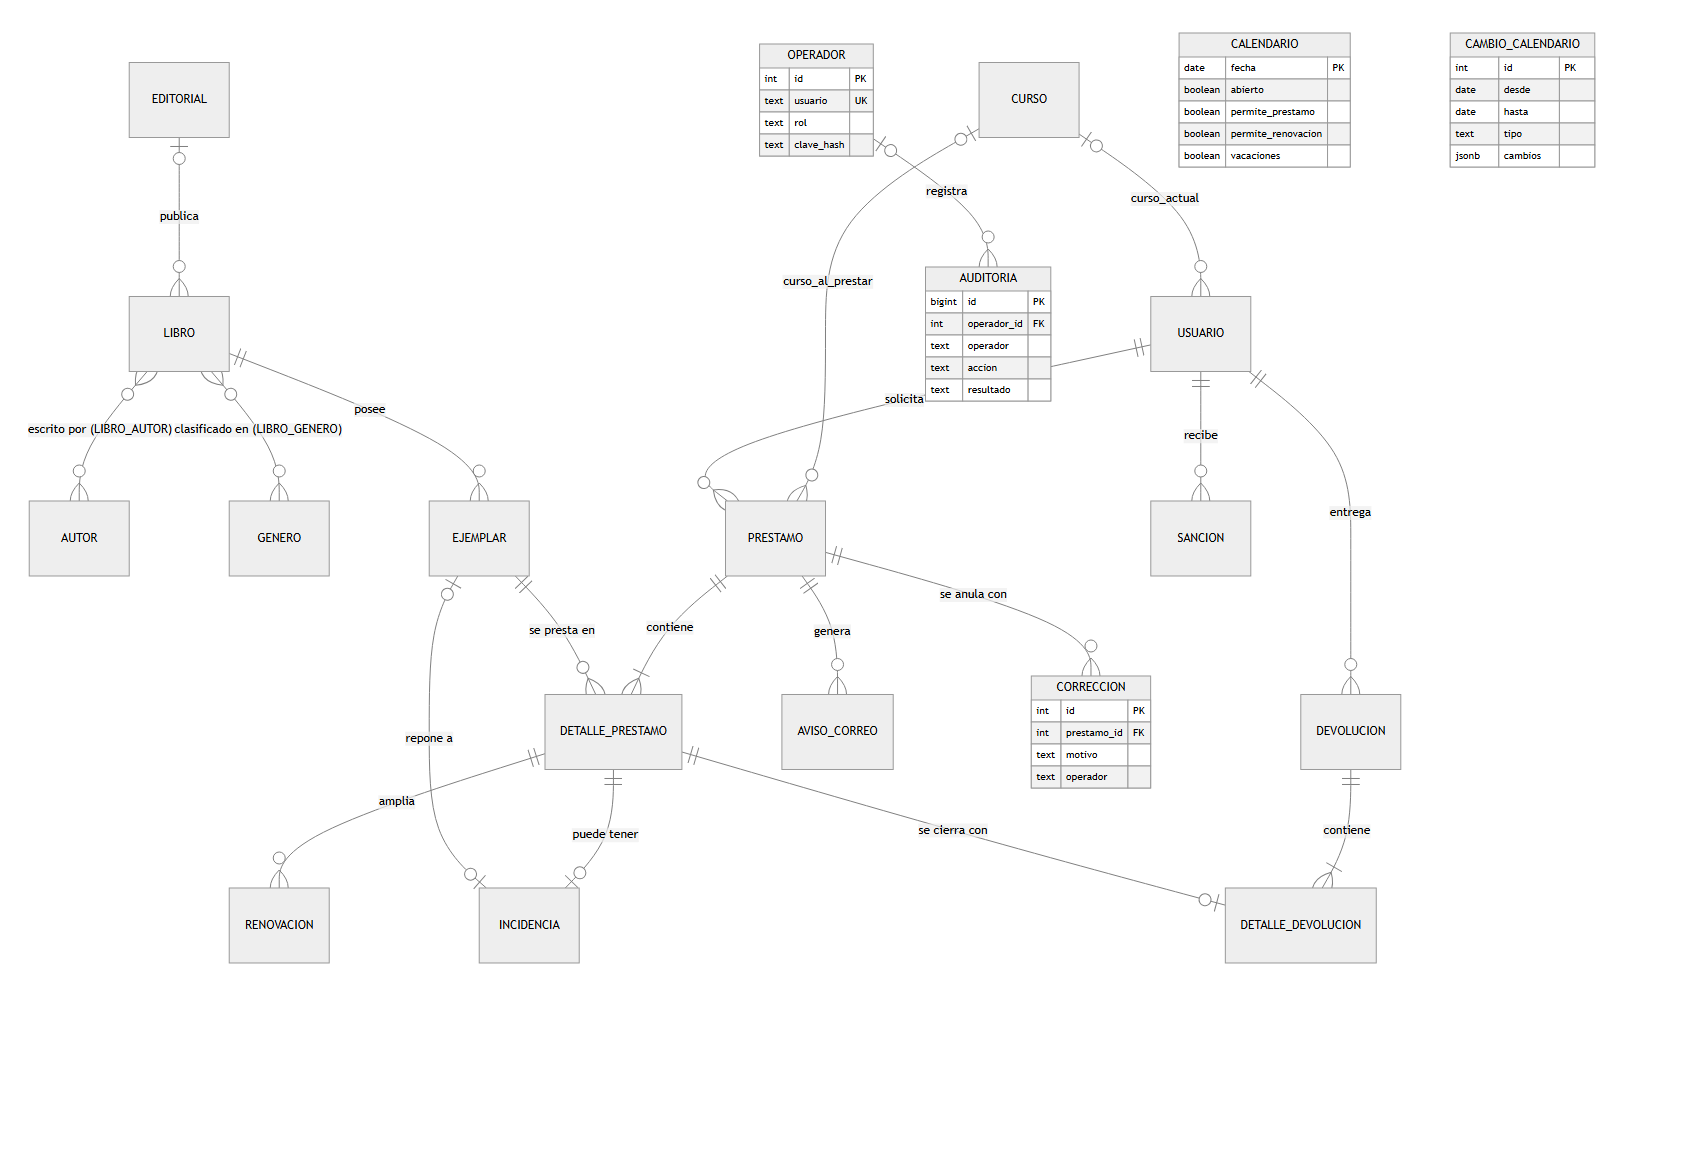
\includegraphics[width=\textwidth,height=0.75\textheight,keepaspectratio]{er.png}
\caption{Diagrama entidad-relación (notación pata de gallo).}
\end{figure}

%------------------------------------------------------------
\subsection{Modelo relacional}

\subsubsection{Aplicación del algoritmo de transformación}
\textbf{Paso 1: entidades fuertes.} Cada entidad fuerte pasa a una tabla con clave primaria sustituta \texttt{id} (\texttt{GENERATED ALWAYS AS IDENTITY}). Las claves naturales se conservan como \texttt{UNIQUE}: \texttt{libro.isbn}, \texttt{ejemplar.codigo}, \texttt{usuario.identificador} (RUT) y \texttt{operador.usuario}. Resultado: \texttt{editorial}, \texttt{autor}, \texttt{genero}, \texttt{libro}, \texttt{ejemplar}, \texttt{curso}, \texttt{usuario}, \texttt{prestamo}, \texttt{devolucion} y \texttt{operador}. \texttt{Calendario} usa la fecha como clave natural.

\textbf{Paso 2: entidades débiles.} \texttt{Renovación}, \texttt{Sanción}, \texttt{AvisoCorreo} y \texttt{Corrección} dependen de su dueño: pasan a tablas con clave foránea obligatoria (\texttt{NOT NULL}) hacia él (\texttt{renovacion.detalle\_id}, \texttt{sancion.usuario\_id}, \texttt{aviso\_correo.prestamo\_id}, \texttt{correccion.prestamo\_id}). Se les dio un \texttt{id} propio para simplificar las referencias.

\textbf{Paso 3: relaciones 1:1.} R7 y R13 son 1:1 opcionales. Se eligió poner la clave foránea con \texttt{UNIQUE} en el lado opcional (\texttt{detalle\_devolucion.detalle\_prestamo\_id}, \texttt{incidencia.detalle\_id}), porque así no hay columnas nulas en \texttt{detalle\_prestamo} y la unicidad garantiza que una copia prestada se devuelve o se declara perdida una sola vez.

\textbf{Paso 4: relaciones 1:N.} La clave foránea va en el lado N: \texttt{libro.editorial\_id}, \texttt{ejemplar.libro\_id}, \texttt{prestamo.usuario\_id}, \texttt{detalle\_prestamo.prestamo\_id}, \texttt{detalle\_devolucion.devolucion\_id}, entre otras. Si el lado 1 es opcional, la columna admite \texttt{NULL} (\texttt{libro.editorial\_id}, \texttt{usuario.curso\_actual\_id}). La participación total «1..N» de un préstamo con sus detalles no se puede expresar con una clave foránea; se impone con un trigger diferido que rechaza un préstamo sin detalles al confirmar la transacción.

\textbf{Paso 5: relaciones N:M.} \texttt{Libro}--\texttt{Autor} pasa a \texttt{libro\_autor(libro\_id, autor\_id)} con clave primaria compuesta por ambas claves foráneas; igual \texttt{libro\_genero(libro\_id, genero\_id)}. La relación préstamo--ejemplar, que tiene atributos propios (vencimiento, renovaciones), queda como la tabla asociativa \texttt{detalle\_prestamo} con \texttt{UNIQUE(prestamo\_id, ejemplar\_id)}.

\textbf{Paso 6: atributos multivaluados.} Los autores y géneros de un libro, que son multivaluados, ya quedaron en tablas propias en el paso 5. Los ejemplares de un préstamo están en \texttt{detalle\_prestamo}, no en columnas \texttt{ejemplar1..3}.

\textbf{Paso 7: relaciones n-arias.} No aplica: todas las relaciones del modelo son binarias. La operación que asocia usuario, préstamo y ejemplar se resolvió con dos relaciones binarias (R4 y R6, a través de \texttt{detalle\_prestamo}).

\subsubsection{Diagrama del modelo relacional}
\begin{figure}[H]
\centering
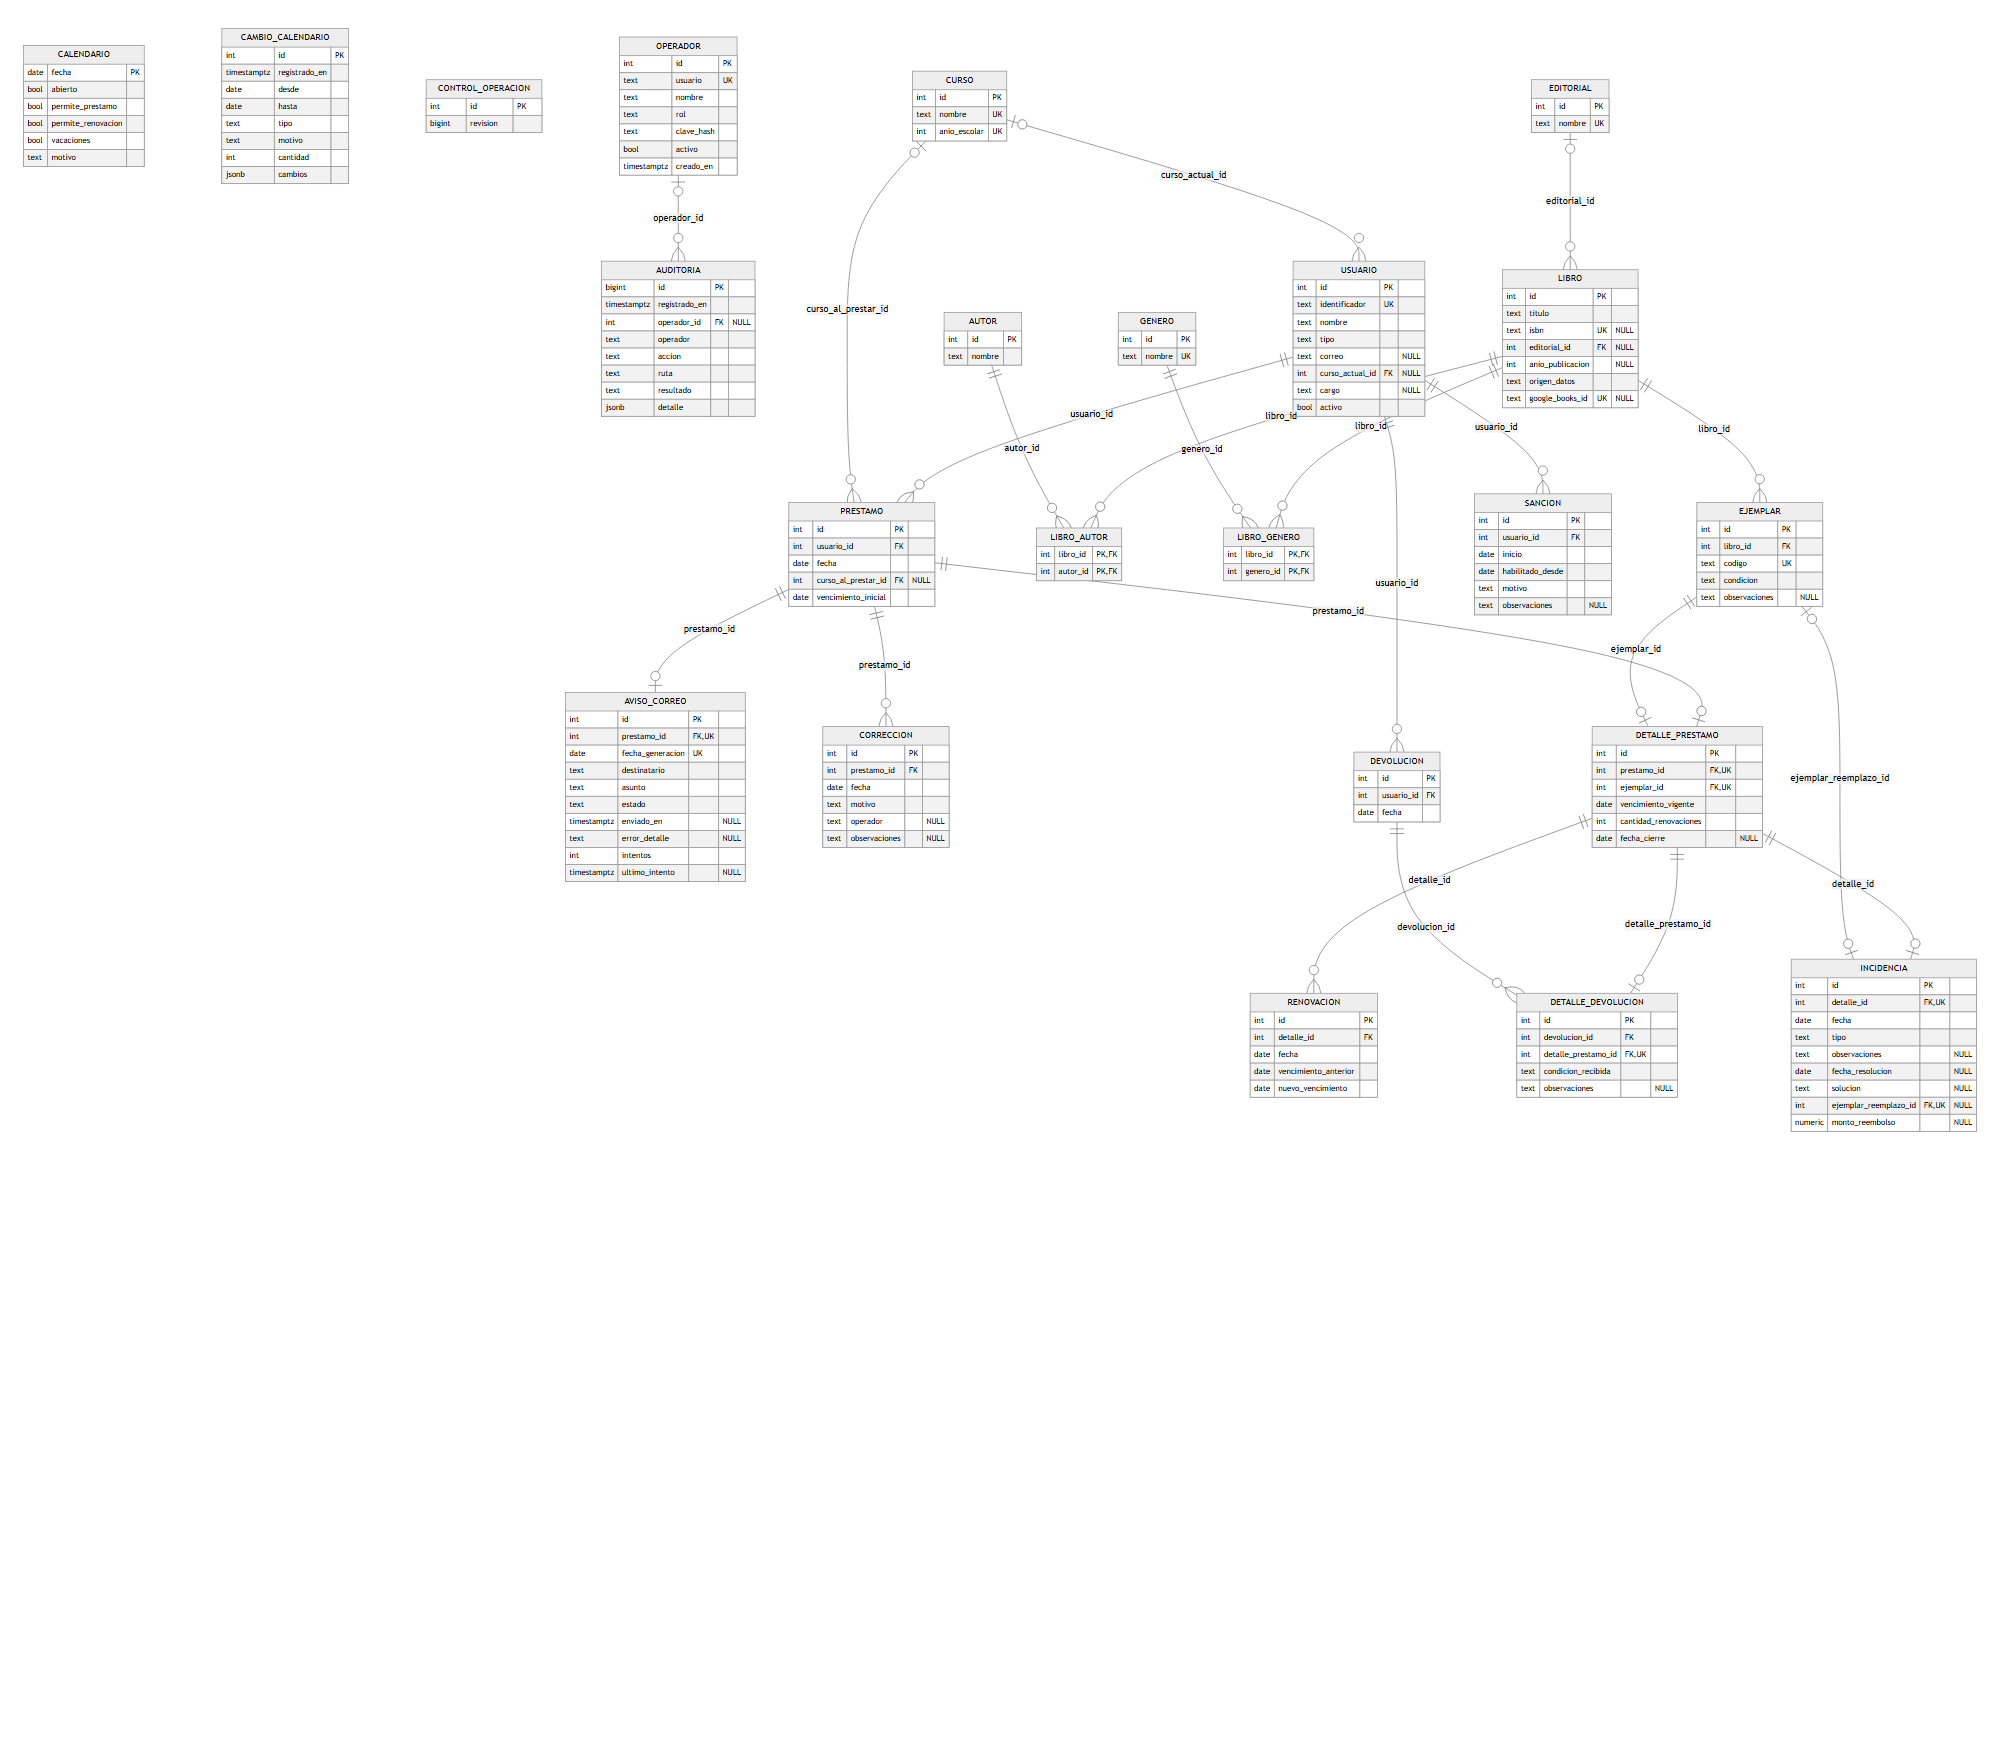
\includegraphics[width=\textwidth,trim=0 600 0 0,clip]{relacional.png}
\caption{Modelo relacional con claves primarias y foráneas marcadas (PK, FK, UK; «NULL» = admite nulos). Generado del catálogo de una base recién creada: 23 tablas y 21 claves foráneas.}
\end{figure}

%------------------------------------------------------------
\subsection{Normalización}

\subsubsection{Forma normal de cada relación}
{\small
\begin{longtable}{@{}p{0.2\textwidth} p{0.13\textwidth} p{0.3\textwidth} l p{0.22\textwidth}@{}}
\caption{Análisis de formas normales por relación.}\\
\toprule
\textbf{Relación} & \textbf{PK} & \textbf{Dependencias funcionales} & \textbf{FN} & \textbf{Justificación}\\
\midrule
\endfirsthead
\caption[]{Análisis de formas normales por relación (continuación).}\\
\toprule
\textbf{Relación} & \textbf{PK} & \textbf{Dependencias funcionales} & \textbf{FN} & \textbf{Justificación}\\
\midrule
\endhead
editorial, genero & id & id $\to$ nombre; nombre $\to$ id & FNBC & Ambos determinantes son claves.\\
autor & id & id $\to$ nombre & FNBC & Se admiten homónimos.\\
libro & id & id $\to$ titulo, isbn, editorial\_id, anio\_publicacion, origen\_datos, google\_books\_id & FNBC & isbn y google\_books\_id son claves candidatas; el nombre de la editorial está en editorial.\\
libro\_autor, libro\_genero & (libro\_id, autor\_id / genero\_id) & Solo triviales & FNBC & Todos los atributos son primos.\\
ejemplar & id & id $\to$ libro\_id, codigo, condicion, observaciones; codigo $\to$ id & FNBC & El título está en libro, no en ejemplar.\\
curso & id & id $\to$ nombre, anio\_escolar; (nombre, anio\_escolar) $\to$ id & FNBC & Ambos determinantes son claves.\\
usuario & id & id $\to$ identificador, nombre, tipo, correo, curso\_actual\_id, cargo, activo & FNBC & El nombre del curso está en curso.\\
prestamo & id & id $\to$ usuario\_id, fecha, curso\_al\_prestar\_id, vencimiento\_inicial & 3FN & curso\_al\_prestar\_id es un hecho histórico, no depende de usuario\_id.\\
detalle\_prestamo & id & id $\to$ prestamo\_id, ejemplar\_id, vencimiento\_vigente, cantidad\_renovaciones, fecha\_cierre & 3FN & Atributos derivados mantenidos por triggers.\\
renovacion & id & id $\to$ detalle\_id, fecha, vencimiento\_anterior, nuevo\_vencimiento & FNBC & ---\\
devolucion & id & id $\to$ usuario\_id, fecha & FNBC & ---\\
detalle\_devolucion & id & id $\to$ devolucion\_id, detalle\_prestamo\_id, condicion\_recibida, observaciones & FNBC & detalle\_prestamo\_id es clave candidata.\\
incidencia & id & id $\to$ detalle\_id, fecha, tipo, solucion, ejemplar\_reemplazo\_id, monto\_reembolso, \ldots & FNBC & detalle\_id es clave candidata.\\
sancion & id & id $\to$ usuario\_id, inicio, habilitado\_desde, motivo & 3FN & habilitado\_desde se guarda como término comunicado.\\
calendario & fecha & fecha $\to$ abierto, permite\_prestamo, permite\_renovacion, vacaciones, motivo & FNBC & ---\\
aviso\_correo & id & id $\to$ todos; (prestamo\_id, fecha\_generacion) $\to$ id & 3FN & destinatario es una instantánea del envío.\\
correccion, operador & id & id $\to$ resto de atributos & FNBC & ---\\
auditoria & id & id $\to$ registrado\_en, operador\_id, operador, accion, ruta, resultado, detalle & 3FN & operador es el nombre en ese momento.\\
\bottomrule
\end{longtable}}

\subsubsection{Proceso de descomposición}
\textbf{1FN.} En el modelo conceptual un libro tiene una lista de autores y de géneros, y un préstamo una lista de hasta tres ejemplares. Esos grupos repetidos se descompusieron en \texttt{libro\_autor}, \texttt{libro\_genero} y \texttt{detalle\_prestamo}, con una fila por valor.

\textbf{2FN.} Una tabla única de préstamos con clave (préstamo, ejemplar) tendría dependencias parciales: usuario, fecha y curso dependen solo del préstamo. Se descompuso en \texttt{prestamo} (cabecera) y \texttt{detalle\_prestamo}; en esta última, \texttt{vencimiento\_vigente} depende de la copia dentro del préstamo, porque cada copia se renueva por su cuenta. Lo mismo para \texttt{devolucion} y \texttt{detalle\_devolucion}.

\textbf{3FN.} Se eliminaron las dependencias transitivas: el título y los autores están en \texttt{libro} y no en \texttt{ejemplar} (ejemplar $\to$ libro $\to$ título); el nombre del curso en \texttt{curso} y no en \texttt{usuario}; el nombre de la editorial en \texttt{editorial} y no en \texttt{libro}; el correo y el nombre del usuario en \texttt{usuario} y no en \texttt{prestamo}.

\textbf{Verificación.} Cada descomposición es sin pérdida, porque el atributo común es clave de una de las partes (por ejemplo, \texttt{prestamo\_id} es clave de \texttt{prestamo}), y conserva las dependencias, porque cada una queda dentro de una sola tabla. Las relaciones marcadas como 3FN y no FNBC lo son por atributos derivados o instantáneas guardados a propósito (redundancia controlada): solo los escriben los triggers y no se pueden modificar a mano.

\subsubsection{Diagrama del modelo normalizado}
El modelo relacional de la Figura~2 ya es el resultado de la normalización: no hubo que descomponer más tablas después de transformarlo. Por eso el diagrama normalizado coincide con él.
\begin{figure}[H]
\centering
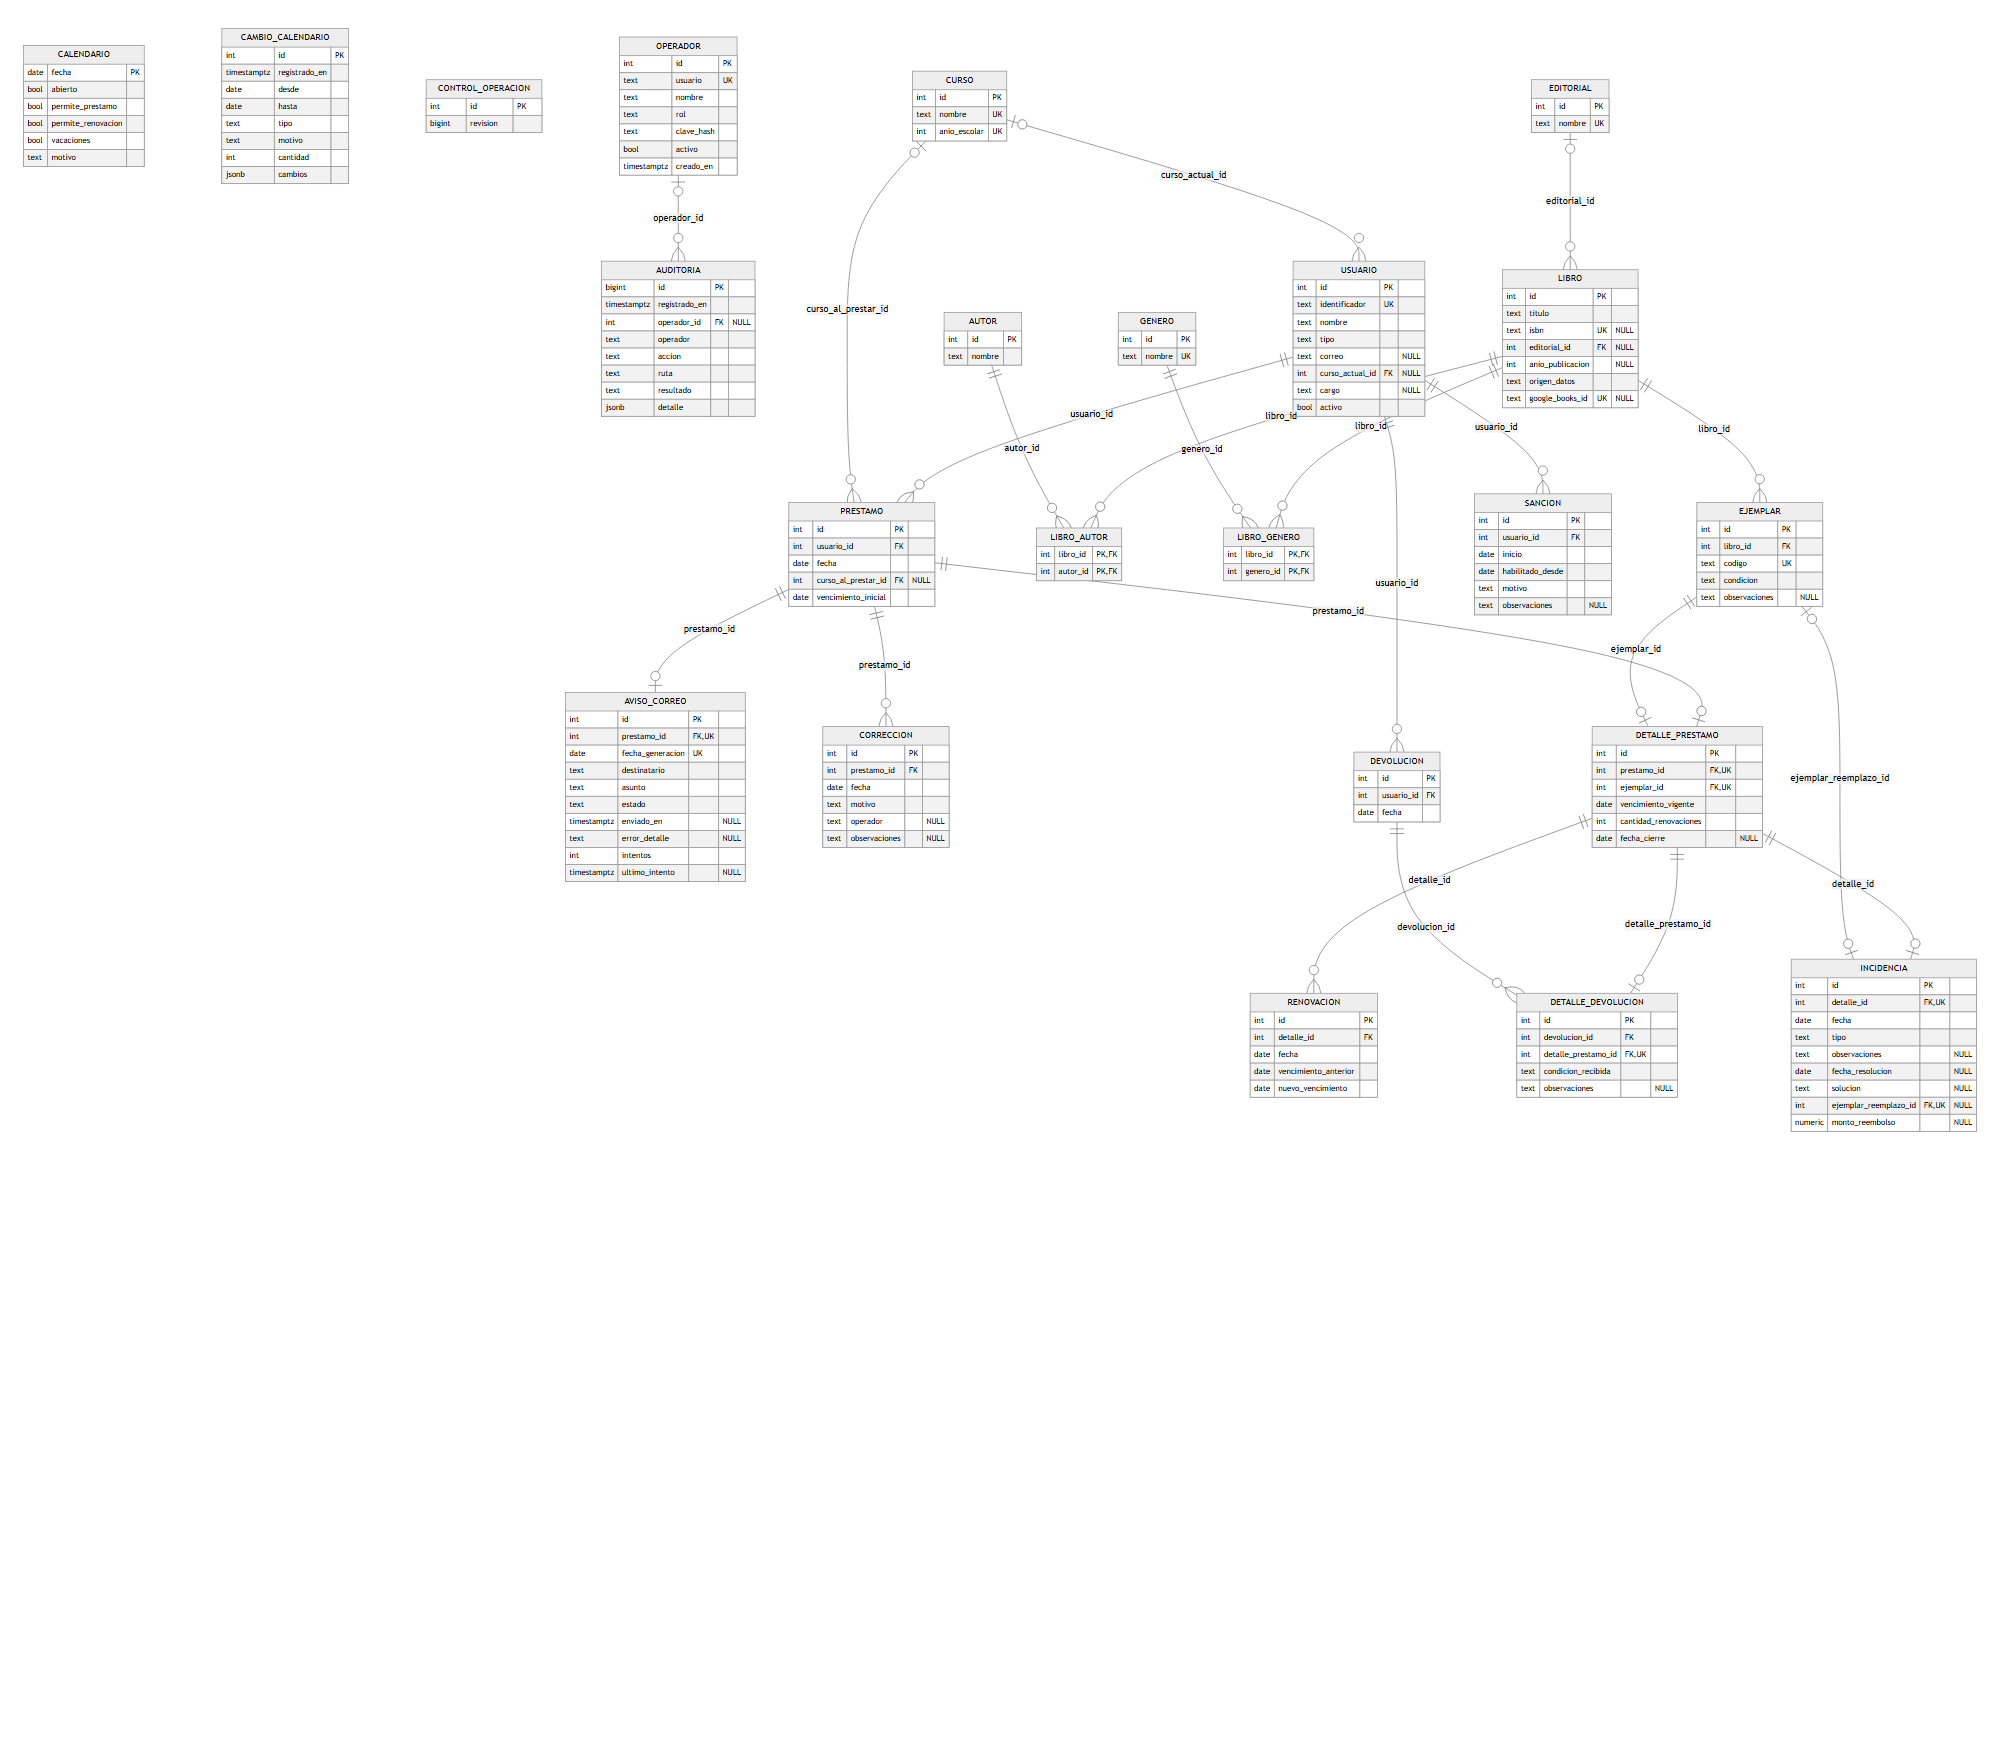
\includegraphics[width=\textwidth,trim=0 600 0 0,clip]{relacional.png}
\caption{Modelo relacional normalizado (3FN, la mayoría de las relaciones en FNBC).}
\end{figure}

%------------------------------------------------------------
\subsection{Modelo físico}

\subsubsection{Motor y herramientas}
El motor es PostgreSQL. El script usa SQL estándar de PostgreSQL y PL/pgSQL, y funciona en un servidor PostgreSQL 16 o superior (cliente \texttt{psql} o pgAdmin). Para que la aplicación funcione sin instalar un servidor, se usa PGlite 0.5.16, que es PostgreSQL compilado para ejecutarse dentro de Node.js 24 y guarda la base en una carpeta local. Todo el esquema vive en el esquema \texttt{biblioteca}.

\subsubsection{Creación de la base y las tablas}
El script completo (\texttt{BibliotecaSigloXXI-scripts.sql}, Anexo~D) crea el esquema, las 23 tablas, los triggers, los procedimientos, los datos de ejemplo y las consultas. Fragmento de la creación de las tablas de préstamo:
\begin{lstlisting}[language=SQL]
CREATE TABLE prestamo (
    id integer GENERATED ALWAYS AS IDENTITY PRIMARY KEY,
    usuario_id integer NOT NULL REFERENCES usuario(id),
    fecha date NOT NULL,
    curso_al_prestar_id integer REFERENCES curso(id),
    vencimiento_inicial date NOT NULL,
    CHECK (vencimiento_inicial > fecha)
);
CREATE TABLE detalle_prestamo (
    id integer GENERATED ALWAYS AS IDENTITY PRIMARY KEY,
    prestamo_id integer NOT NULL REFERENCES prestamo(id),
    ejemplar_id integer NOT NULL REFERENCES ejemplar(id),
    vencimiento_vigente date NOT NULL,
    cantidad_renovaciones integer NOT NULL DEFAULT 0
        CHECK (cantidad_renovaciones BETWEEN 0 AND 2),   -- RN05
    fecha_cierre date,
    UNIQUE (prestamo_id, ejemplar_id)
);
-- RN04: un solo préstamo abierto por ejemplar
CREATE UNIQUE INDEX ejemplar_un_prestamo_abierto
    ON detalle_prestamo(ejemplar_id) WHERE fecha_cierre IS NULL;
\end{lstlisting}

\subsubsection{Poblamiento}
Todos los datos son inventados: los libros se llaman «Obra ficticia 1» a «Obra ficticia 12» y los correos usan el dominio reservado \texttt{example.invalid}. Volumen: 12 libros, 37 ejemplares, 3 autores, 3 géneros, 2 editoriales, 20 cursos (Pre-kínder a 8.º básico de 2026 y 2027), 12 usuarios (10 estudiantes, 1 docente y 1 asistente), 6 préstamos con 9 detalles, 5 devoluciones, 1 renovación, 2 incidencias, 1 sanción, 1 aviso y 730 días de calendario (2026--2027). El criterio fue cubrir cada caso de negocio con al menos un registro: préstamos abiertos, devueltos y atrasados, una devolución parcial, una renovación, una pérdida, un daño, una sanción y un feriado. El poblamiento incluye la traza de los ejemplares A, B y C descrita en la Sección~3.2.2.

\subsubsection{Instrucciones para levantar la base desde cero}
\begin{enumerate}[nosep]
\item Instalar PostgreSQL 16 o superior (o usar la aplicación, que trae PGlite y no requiere instalar un servidor).
\item Crear una base vacía y ejecutar el script: \texttt{createdb biblioteca} y luego \texttt{psql -d biblioteca -f BibliotecaSigloXXI-scripts.sql}.
\item Verificar con una consulta de ejemplo: \texttt{SELECT count(*) FROM biblioteca.curso;} debe devolver 20, y \texttt{SELECT * FROM biblioteca.v\_disponibilidad;} lista los ejemplares disponibles.
\end{enumerate}
Con la aplicación: \texttt{npm install}, \texttt{npm run db:init} (crea la base con los mismos archivos SQL) y \texttt{npm start}.

%------------------------------------------------------------
\subsection{Triggers y procedimientos almacenados}

\subsubsection{Trigger que hace cumplir una restricción de integridad}
El trigger \texttt{validar\_detalle} se dispara antes de insertar cada fila en \texttt{detalle\_prestamo} y protege RN02 (máximo tres ejemplares simultáneos por persona) y RN10 (máximo tres por operación). También rechaza ejemplares perdidos o dañados y usuarios bloqueados (RN13, RN14). Una restricción declarativa no basta: \texttt{CHECK} solo ve la fila que se inserta, y aquí hay que contar filas de otros préstamos del mismo usuario que siguen abiertos.
\begin{lstlisting}[language=SQL]
CREATE FUNCTION validar_detalle() RETURNS trigger LANGUAGE plpgsql AS $$
DECLARE p biblioteca.prestamo%ROWTYPE; estado text;
BEGIN
  SELECT * INTO STRICT p FROM biblioteca.prestamo WHERE id=NEW.prestamo_id;
  SELECT condicion INTO STRICT estado FROM biblioteca.ejemplar WHERE id=NEW.ejemplar_id;
  IF estado NOT IN ('bueno','desgastado') THEN
    RAISE EXCEPTION 'Ejemplar no disponible por su condición'; END IF;
  IF EXISTS (SELECT 1 FROM biblioteca.motivos_bloqueo(p.usuario_id,p.fecha)) THEN
    RAISE EXCEPTION 'Usuario bloqueado para préstamos'; END IF;
  IF (SELECT count(*) FROM biblioteca.detalle_prestamo dp
      JOIN biblioteca.prestamo op ON op.id=dp.prestamo_id
      WHERE op.usuario_id=p.usuario_id AND dp.fecha_cierre IS NULL)>=3 THEN
    RAISE EXCEPTION 'Máximo tres ejemplares simultáneos por usuario'; END IF;
  NEW.vencimiento_vigente := p.vencimiento_inicial;
  NEW.cantidad_renovaciones := 0;
  RETURN NEW;
END $$;
CREATE TRIGGER validar_detalle BEFORE INSERT ON detalle_prestamo
  FOR EACH ROW EXECUTE FUNCTION validar_detalle();
\end{lstlisting}

\subsubsection{Trigger que mantiene un atributo calculado}
El trigger \texttt{actualizar\_vencimiento} mantiene dos atributos calculados de \texttt{detalle\_prestamo}: \texttt{vencimiento\_vigente} y \texttt{cantidad\_renovaciones}. Ambos dependen de las filas de \texttt{renovacion} de ese detalle (RN05, RN06). Se dispara después de cada \texttt{INSERT} en \texttt{renovacion}: copia el nuevo vencimiento, ya calculado en días hábiles según el calendario, y suma uno al contador. Otro trigger impide modificar estos atributos a mano.
\begin{lstlisting}[language=SQL]
CREATE FUNCTION actualizar_vencimiento() RETURNS trigger LANGUAGE plpgsql AS $$
BEGIN
  UPDATE biblioteca.detalle_prestamo
     SET vencimiento_vigente = NEW.nuevo_vencimiento,
         cantidad_renovaciones = cantidad_renovaciones + 1
   WHERE id = NEW.detalle_id;
  RETURN NEW;
END $$;
CREATE TRIGGER actualizar_vencimiento AFTER INSERT ON renovacion
  FOR EACH ROW EXECUTE FUNCTION actualizar_vencimiento();
\end{lstlisting}

\subsubsection{Procedimiento almacenado de KPIs}
\begin{table}[H]
\centering
\caption{Indicadores anuales del caso.}
\small
\begin{tabularx}{\textwidth}{l Y l Y}
\toprule
\textbf{KPI} & \textbf{Definición y unidad de conteo} & \textbf{Origen} & \textbf{Decisión que sustenta}\\
\midrule
KPI 1: Préstamos por curso & Operaciones de préstamo según el curso registrado al retirar los libros. Tres ejemplares retirados juntos cuentan como un préstamo. & Presentación de avance & Ver qué cursos usan menos la biblioteca, para orientar actividades de fomento lector.\\
KPI 2: Libros más prestados & Cantidad de ejemplares retirados de cada libro durante el año. Las renovaciones no agregan préstamos nuevos. & Presentación de avance & Identificar los títulos más utilizados, para decidir qué libros conviene comprar en más copias.\\
\bottomrule
\end{tabularx}
\end{table}

La biblioteca revisa sus estadísticas anualmente. Los indicadores se calculan con los movimientos de la biblioteca, no con datos de Google Books.

El procedimiento \texttt{sp\_kpis\_anuales} recibe un año y devuelve los dos indicadores en formato JSON. El KPI 1 agrupa por \texttt{curso\_al\_prestar\_id}, de modo que el resultado no cambia cuando un estudiante pasa de curso. El KPI 2 cuenta filas de \texttt{detalle\_prestamo}, así que las renovaciones no suman.
\begin{lstlisting}[language=SQL]
CREATE PROCEDURE sp_kpis_anuales(IN p_anio integer,
    INOUT p_por_curso jsonb DEFAULT NULL,
    INOUT p_libros_mas_prestados jsonb DEFAULT NULL)
LANGUAGE plpgsql AS $$
BEGIN
  SELECT coalesce(jsonb_agg(to_jsonb(q) ORDER BY q.prestamos DESC),'[]')
    INTO p_por_curso FROM (
    SELECT c.id AS curso_id, coalesce(c.nombre,'Sin curso') AS curso,
           count(*) AS prestamos
    FROM biblioteca.prestamo p
    LEFT JOIN biblioteca.curso c ON c.id = p.curso_al_prestar_id
    WHERE p.fecha >= make_date(p_anio,1,1) AND p.fecha < make_date(p_anio+1,1,1)
    GROUP BY c.id, c.nombre) q;
  SELECT coalesce(jsonb_agg(to_jsonb(q) ORDER BY q.ejemplares_prestados DESC),'[]')
    INTO p_libros_mas_prestados FROM (
    SELECT l.id AS libro_id, l.titulo, count(*) AS ejemplares_prestados
    FROM biblioteca.prestamo p
    JOIN biblioteca.detalle_prestamo d ON d.prestamo_id = p.id
    JOIN biblioteca.ejemplar e ON e.id = d.ejemplar_id
    JOIN biblioteca.libro l ON l.id = e.libro_id
    WHERE p.fecha >= make_date(p_anio,1,1) AND p.fecha < make_date(p_anio+1,1,1)
    GROUP BY l.id, l.titulo) q;
END $$;
-- Uso: CALL biblioteca.sp_kpis_anuales(2026);
\end{lstlisting}

\subsubsection{Procedimiento almacenado con actualización y rollback}
El procedimiento \texttt{sp\_actualizar\_correo} actualiza el correo de un usuario en la tabla \texttt{usuario}. Si el usuario no existe, lanza un error y PostgreSQL revierte la transacción. Si la bibliotecaria no confirma el cambio (\texttt{p\_confirmar = false}), el procedimiento ejecuta \texttt{ROLLBACK} y el correo anterior se mantiene; si lo confirma, ejecuta \texttt{COMMIT}. Se eligió el correo porque es el dato al que llegan los avisos de atraso: un cambio no revisado dejaría al estudiante sin avisos.
\begin{lstlisting}[language=SQL]
CREATE PROCEDURE sp_actualizar_correo(IN p_usuario integer,
    IN p_correo text, IN p_confirmar boolean)
LANGUAGE plpgsql AS $$
BEGIN
  IF p_confirmar IS NULL THEN RAISE EXCEPTION 'Indique confirmar o revertir'; END IF;
  UPDATE biblioteca.usuario SET correo = p_correo WHERE id = p_usuario;
  IF NOT FOUND THEN RAISE EXCEPTION 'Usuario inexistente'; END IF;
  IF p_confirmar THEN COMMIT; ELSE ROLLBACK; END IF;
END $$;
\end{lstlisting}
Además de estos, la base tiene los procedimientos de operación \texttt{sp\_prestar}, \texttt{sp\_renovar}, \texttt{sp\_devolver}, \texttt{sp\_registrar\_incidencia}, \texttt{sp\_resolver\_incidencia}, \texttt{sp\_sancionar\_conducta}, \texttt{sp\_anular\_prestamo} y \texttt{sp\_preparar\_avisos}.

%------------------------------------------------------------
\subsection{API de consulta}

\subsubsection{Arquitectura y tecnologías}
La arquitectura propuesta es la siguiente: la bibliotecaria ingresa el ISBN en el registro de libros; un módulo de consulta busca y prepara los datos para revisión en la Google Books API; después de revisarlos, se guardan en la base de la biblioteca (catálogo, ejemplares y movimientos). La conexión se realiza mediante la aplicación y la API. La API está escrita en JavaScript sobre Node.js 24, con el módulo \texttt{http} estándar y sin framework. Al iniciar abre la base con PGlite (o con un servidor PostgreSQL) y mantiene esa conexión; cada ruta ejecuta una consulta \texttt{SELECT} o un \texttt{CALL} con parámetros (\texttt{\$1}, \texttt{\$2}, \ldots) y responde en JSON. La interfaz web (HTML y JavaScript en la carpeta \texttt{web/}) consume esas rutas desde el navegador. Las rutas exigen una sesión iniciada (cookie) y, para modificar datos, un encabezado contra falsificación de peticiones; el rol \texttt{consulta} solo puede leer. La consulta a Google Books se hace desde el servidor, con la clave guardada en el archivo \texttt{.env}, que no se publica.

\subsubsection{Endpoints}
\begin{longtable}{@{}l l p{0.55\textwidth}@{}}
\caption{Endpoints principales de la API.}\\
\toprule
\textbf{Método} & \textbf{Ruta} & \textbf{Descripción}\\
\midrule
\endfirsthead
\caption[]{Endpoints principales de la API (continuación).}\\
\toprule
\textbf{Método} & \textbf{Ruta} & \textbf{Descripción}\\
\midrule
\endhead
GET & \texttt{/api/libros} & Catálogo con editorial, autores, géneros y ejemplares (filtro por texto).\\
GET & \texttt{/api/libros/isbn?isbn=} & Datos del libro en Google Books para revisión antes de guardar.\\
GET & \texttt{/api/ejemplares?disponibles=1} & Ejemplares disponibles (vista \texttt{v\_disponibilidad}).\\
GET & \texttt{/api/usuarios} & Usuarios con curso, préstamos abiertos y bloqueos.\\
GET & \texttt{/api/pendientes} & Préstamos pendientes y atrasados, con días de atraso.\\
GET & \texttt{/api/estadisticas?anio=} & KPIs anuales (llama a \texttt{sp\_kpis\_anuales}).\\
GET & \texttt{/api/resumen}, \texttt{/api/contexto} & Totales del panel inicial, cursos y fecha de atención.\\
GET & \texttt{/api/calendario?mes=} & Días de atención del mes.\\
GET & \texttt{/api/avisos}, \texttt{/api/auditoria} & Avisos de atraso y registro de operaciones.\\
POST & \texttt{/api/prestamos} & Registra un préstamo (\texttt{sp\_prestar}).\\
POST & \texttt{/api/renovaciones}, \texttt{/api/devoluciones} & Renueva o devuelve ejemplares.\\
POST & \texttt{/api/libros}, \texttt{/api/ejemplares}, \texttt{/api/usuarios} & Registra catálogo y usuarios.\\
POST & \texttt{/api/incidencias}, \texttt{/api/sanciones}, \texttt{/api/anulaciones} & Pérdidas y daños, sanciones y correcciones.\\
POST & \texttt{/api/sesion} & Inicia sesión.\\
\bottomrule
\end{longtable}

\subsubsection{Instrucciones de ejecución}
\begin{enumerate}[nosep]
\item Instalar Node.js 20.12 o superior (se usó la versión 24) y, en la carpeta del proyecto, ejecutar \texttt{npm install}.
\item Crear la base con \texttt{npm run db:init}. Para usar un servidor PostgreSQL en vez de PGlite, ejecutar antes el script SQL en ese servidor (README, sección «Ejecutar en un servidor PostgreSQL»). Opcional: poner la clave de Google Books en \texttt{.env}.
\item Levantar la API con \texttt{npm start} y abrir \url{http://localhost:3000}. La primera vez se crea la cuenta de administración.
\end{enumerate}
El documento \texttt{BibliotecaSigloXXI-api.pdf} muestra cada pantalla y cada llamada a la API con capturas, en lugar del video.

%------------------------------------------------------------
\section{Resultados}

\subsection{Pruebas}

\subsubsection{Pruebas del modelo físico}

Todas las pruebas se ejecutaron sobre una base recién creada con el script de entrega. La salida completa de cada caso está en \texttt{BibliotecaSigloXXI-evidencias.pdf}, y las capturas de la API en \texttt{BibliotecaSigloXXI-api.pdf}. Además, el proyecto tiene una batería automática (\texttt{npm test}) de 119 pruebas sobre la base, la API, los respaldos, los avisos, Google Books y la seguridad; en la última ejecución pasaron las 119, sin fallos.

\textbf{Prueba P1 --- crear\_bd: Creación de la base y las tablas}
\begin{itemize}[nosep]
\item \textbf{Objetivo.} Verificar que el script crea el esquema completo sin errores.
\item \textbf{Descripción.} Ejecutar \texttt{BibliotecaSigloXXI-scripts.sql} en una base vacía y consultar el catálogo del motor (\texttt{information\_schema}).
\item \textbf{Evidencia.} El script terminó sin errores y el catálogo lista 23 tablas y 21 claves foráneas en el esquema \texttt{biblioteca}; el diagrama de la Figura~2 se generó a partir de ese catálogo.
\item \textbf{Análisis.} El modelo físico coincide con el modelo relacional diseñado: cada tabla y cada clave foránea del diagrama existen en la base.
\end{itemize}

\textbf{Prueba P2 --- poblar\_bd: Poblamiento}
\begin{itemize}[nosep]
\item \textbf{Objetivo.} Comprobar que los datos de ejemplo se cargan respetando todas las restricciones.
\item \textbf{Descripción.} Contar las filas de cada tabla después de ejecutar el script.
\item \textbf{Evidencia.} 12 libros, 37 ejemplares, 20 cursos, 12 usuarios, 6 préstamos con 9 detalles, 5 devoluciones, 1 renovación, 2 incidencias, 1 sanción y 730 días de calendario (Sección~3.5.3). En P-08 de las evidencias: 10 cursos por año (Pre-kínder a 8.º básico) en 2026 y 2027.
\item \textbf{Análisis.} Los datos pasaron por los mismos triggers que una operación real, así que el poblamiento también prueba que las reglas aceptan los casos válidos.
\end{itemize}

\textbf{Prueba P3 --- levantar\_desde\_cero: Instrucciones reproducibles}
\begin{itemize}[nosep]
\item \textbf{Objetivo.} Confirmar que las instrucciones de la Sección~3.5.4 bastan para levantar la base.
\item \textbf{Descripción.} Seguir los pasos en una carpeta nueva y volver a ejecutar la función que crea los cursos.
\item \textbf{Evidencia.} \texttt{SELECT asegurar\_cursos\_colegio(2026)} devuelve 0 cursos creados la segunda vez (evidencias, P-08). Las capturas de la API (\texttt{BibliotecaSigloXXI-api.pdf}) se tomaron sobre una base levantada desde cero.
\item \textbf{Análisis.} La creación es reproducible y repetible: volver a ejecutar la inicialización no duplica datos.
\end{itemize}

\subsubsection{Pruebas de triggers y procedimientos almacenados}

\textbf{Prueba P4 --- trg\_integridad: Trigger de integridad}
\begin{itemize}[nosep]
\item \textbf{Objetivo.} Verificar que la base rechaza préstamos que violan RN02, RN04 y RN10.
\item \textbf{Descripción.} 1. Dato válido aceptado: préstamo de los ejemplares 1 y 2 al usuario 7 desde la API (respuesta 201). 2. Datos que violan la regla: prestar cuatro ejemplares al usuario 8, y prestar el ejemplar 16, que ya está prestado.
\item \textbf{Evidencia.} \texttt{CALL sp\_prestar(8, ARRAY[25,26,27,28], '2026-11-19')} fue rechazado con «Seleccione de uno a tres ejemplares distintos» y el usuario quedó con 0 préstamos. \texttt{CALL sp\_prestar(9, ARRAY[16], '2026-11-19')} fue rechazado por el índice único \texttt{ejemplar\_un\_prestamo\_abierto} (evidencias P-01 y P-02).
\item \textbf{Código.} Trigger \texttt{validar\_detalle} (Sección~3.6.1) e índice único parcial (Sección~3.5.2).
\item \textbf{Análisis.} La operación se rechaza completa, sin dejar un préstamo a medias. Como la regla vive en la base, se cumple aunque la petición no venga de la aplicación.
\end{itemize}

\textbf{Prueba P5 --- trg\_calculado: Trigger de atributo calculado}
\begin{itemize}[nosep]
\item \textbf{Objetivo.} Verificar que una renovación actualiza el vencimiento vigente y el contador de renovaciones.
\item \textbf{Descripción.} Prestar el ejemplar 25 el lunes 02-11-2026, consultar el detalle, renovarlo el 04-11-2026 (antes del vencimiento) y volver a consultar.
\item \textbf{Evidencia.} Antes: detalle 11, vencimiento 2026-11-05, 0 renovaciones. Después de \texttt{CALL sp\_renovar(ARRAY[11], '2026-11-04')}: vencimiento 2026-11-10, 1 renovación (evidencias P-04).
\item \textbf{Código.} Trigger \texttt{actualizar\_vencimiento} (Sección~3.6.2).
\item \textbf{Análisis.} El nuevo vencimiento suma tres días hábiles desde el vencimiento vigente (jueves 5 $\to$ martes 10, sin el fin de semana), como piden RN06 y RN16. El trigger mantiene ambos atributos sin intervención manual.
\end{itemize}

\textbf{Prueba P6 --- sp\_kpis: Procedimiento almacenado de KPIs}
\begin{itemize}[nosep]
\item \textbf{Objetivo.} Obtener los dos indicadores anuales definidos.
\item \textbf{Descripción.} Ejecutar \texttt{CALL sp\_kpis\_anuales(2026)} sobre los datos de ejemplo.
\item \textbf{Evidencia.} Préstamos por curso: 5.º básico 3, 6.º básico 3 y sin curso (docentes y asistentes) 1. Libros más prestados: «Obra ficticia 1» con 2 ejemplares y las obras 2 a 9 con 1 cada una (evidencias P-06). La pantalla de estadísticas de la API muestra el mismo cálculo (Figura~\ref{fig:api-estadisticas}).
\item \textbf{Código.} Procedimiento \texttt{sp\_kpis\_anuales} (Sección~3.6.3).
\item \textbf{Análisis.} El total por curso (7) coincide con las operaciones de préstamo de 2026 y no con los ejemplares, que es la unidad definida para el KPI 1.
\end{itemize}

\textbf{Prueba P7 --- sp\_rollback: Procedimiento con actualización y rollback}
\begin{itemize}[nosep]
\item \textbf{Objetivo.} Mostrar que el procedimiento confirma o revierte la actualización.
\item \textbf{Descripción.} Cambiar el correo del usuario 1 con \texttt{p\_confirmar = false}, consultar, repetir con \texttt{true} y volver a consultar.
\item \textbf{Evidencia.} Con \texttt{false} el correo siguió siendo \texttt{estudiante1@example.invalid}; con \texttt{true} quedó \texttt{confirmado@example.invalid} (evidencias P-07).
\item \textbf{Código.} Procedimiento \texttt{sp\_actualizar\_correo} (Sección~3.6.4).
\item \textbf{Análisis.} \texttt{ROLLBACK} deshace el \texttt{UPDATE} ya ejecutado y \texttt{COMMIT} lo deja permanente.
\end{itemize}

\subsubsection{Prueba de la API}

\textbf{Prueba P8 --- api\_select: API de consulta}
\begin{itemize}[nosep]
\item \textbf{Objetivo.} Verificar que la API expone las consultas de la base al navegador y respeta las reglas.
\item \textbf{Descripción.} Levantar la API con datos de ejemplo y llamar a sus rutas: sin sesión, creando la cuenta inicial, consultando ejemplares disponibles y estadísticas, y registrando un préstamo válido y uno inválido.
\item \textbf{Evidencia.} Sin sesión: 401. Cuenta inicial: 201. \texttt{GET /api/ejemplares?disponibles=1}, \texttt{GET /api/estadisticas} y \texttt{GET /api/auditoria}: 200 con datos en JSON. Préstamo de 4 ejemplares: 400 «Seleccione entre uno y tres ejemplares». Préstamo válido: 201. Las Figuras~\ref{fig:api-prestamo} a~\ref{fig:api-admin} muestran tres de las pantallas; las 11 están en \texttt{BibliotecaSigloXXI-api.pdf}.
\item \textbf{Análisis.} La API devuelve los resultados de las consultas y transmite los rechazos de la base como errores comprensibles, sin exponer el SQL.
\end{itemize}

\begin{figure}[htbp]
\centering
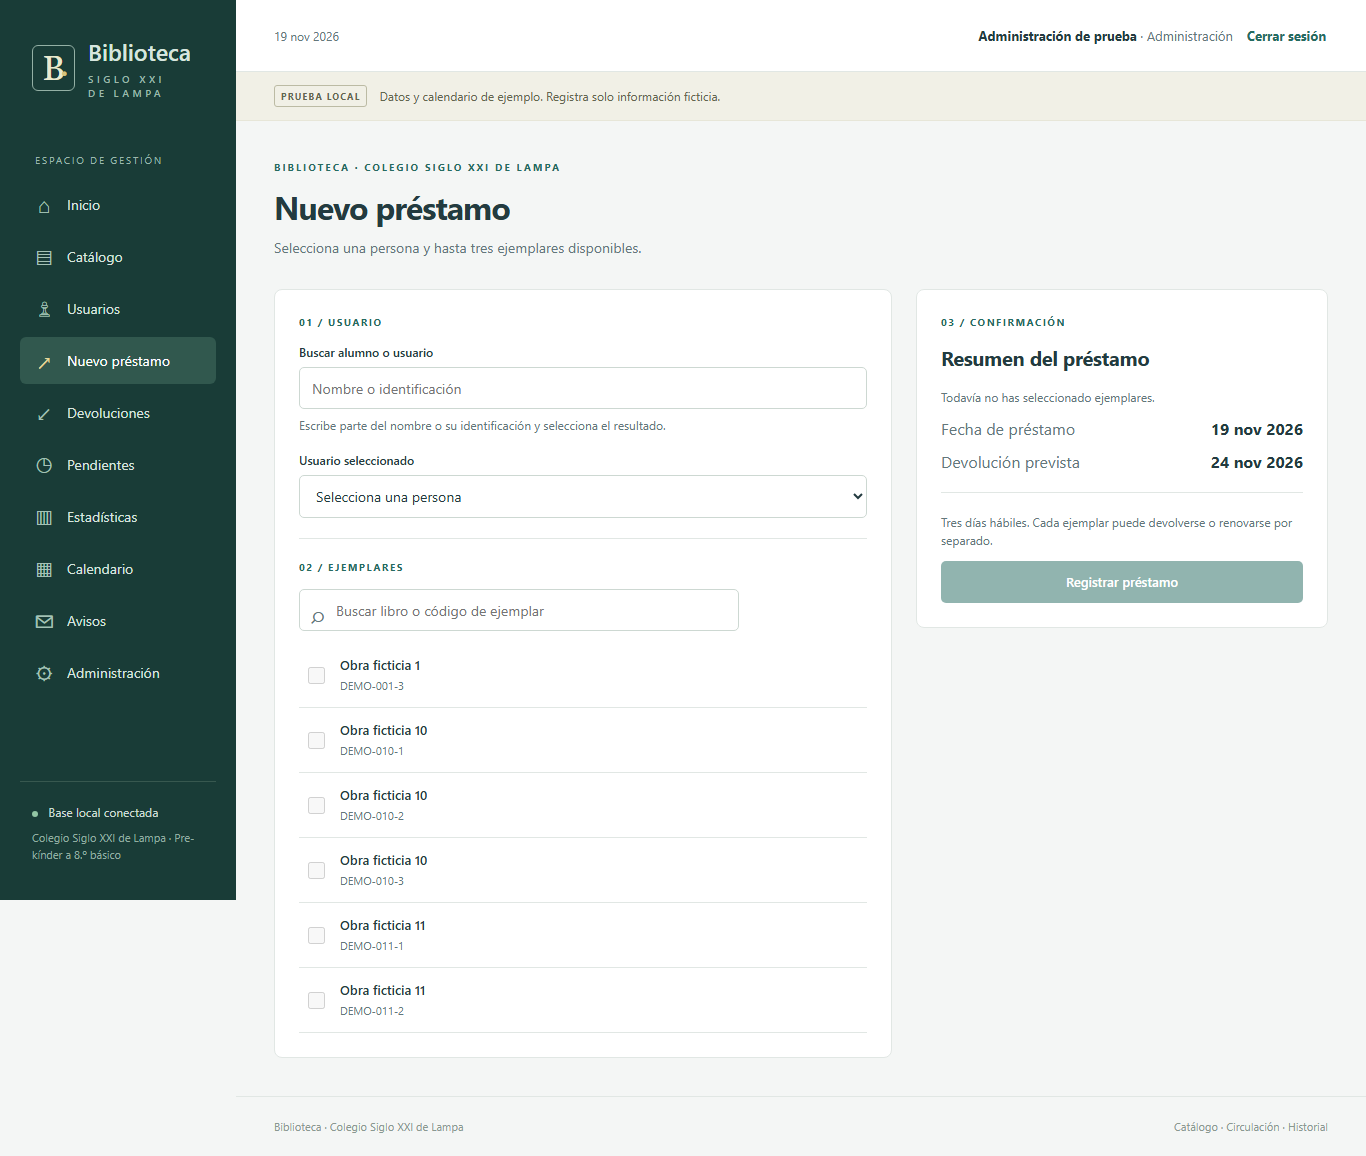
\includegraphics[width=0.85\textwidth]{api-prestamo.png}
\caption{Pantalla de nuevo préstamo. La lista viene de \texttt{GET /api/ejemplares?disponibles=1} y la devolución prevista suma tres días hábiles (RN03).}
\label{fig:api-prestamo}
\end{figure}

\begin{figure}[htbp]
\centering
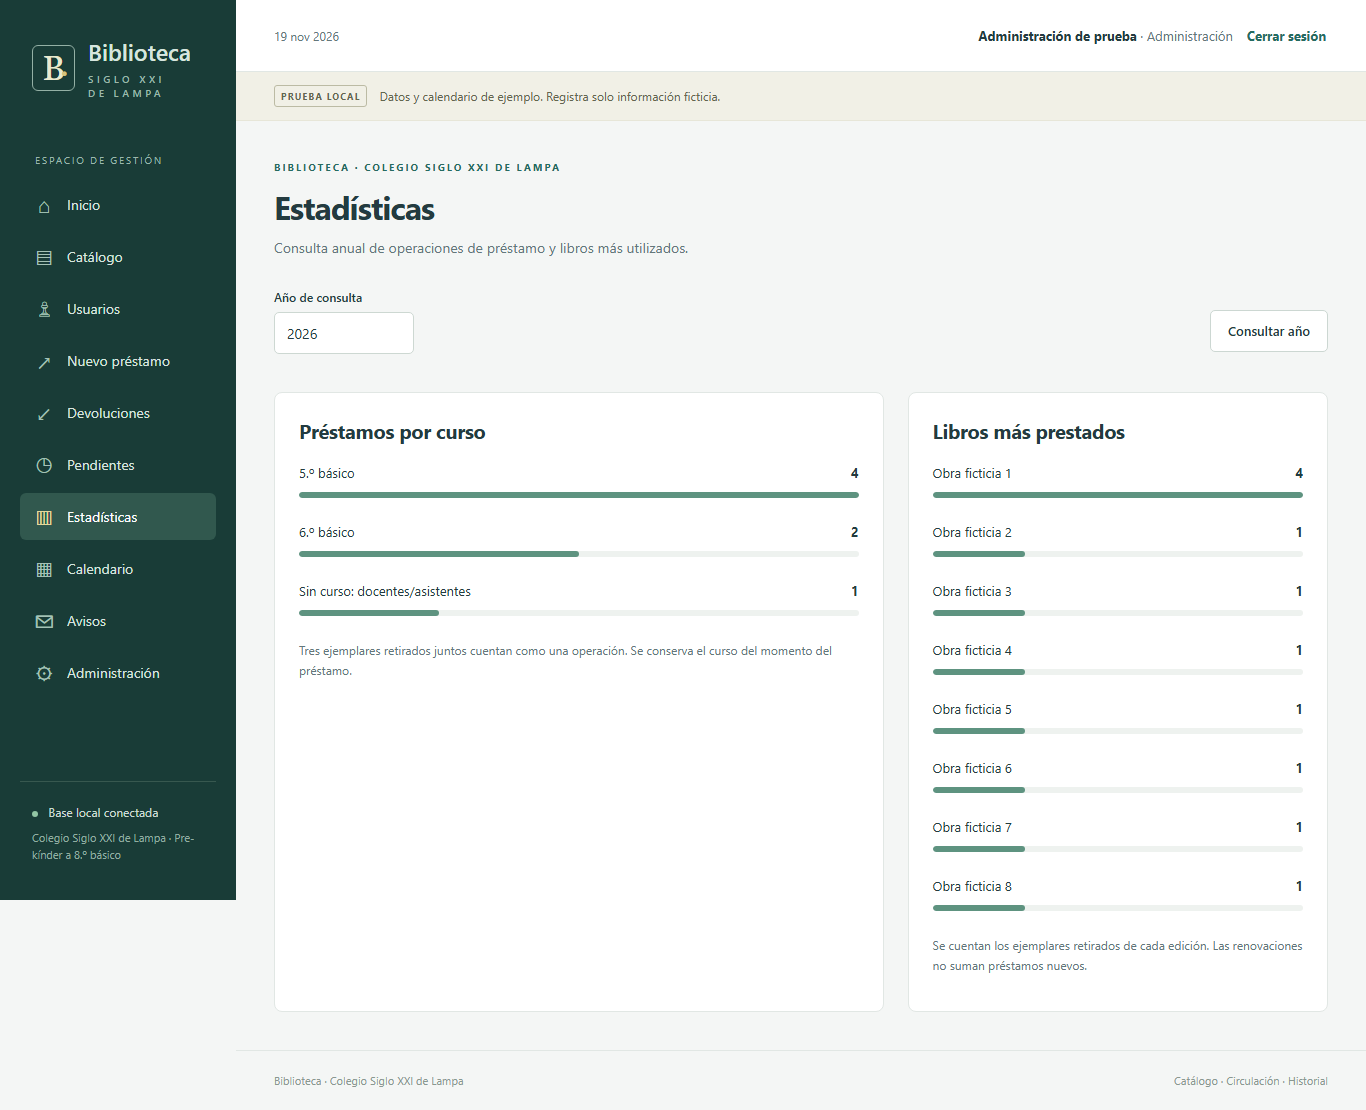
\includegraphics[width=0.85\textwidth]{api-estadisticas.png}
\caption{Pantalla de estadísticas (\texttt{GET /api/estadisticas}, que llama a \texttt{sp\_kpis\_anuales}). Los números difieren de P6 porque cada base recibió préstamos de prueba distintos: P6 incluye el préstamo de P5 (usuario 8, 6.º básico) y esta captura incluye el préstamo válido de P8 (ejemplares 1 y 2 de «Obra ficticia 1» al usuario 7, de 5.º básico).}
\label{fig:api-estadisticas}
\end{figure}

\begin{figure}[htbp]
\centering
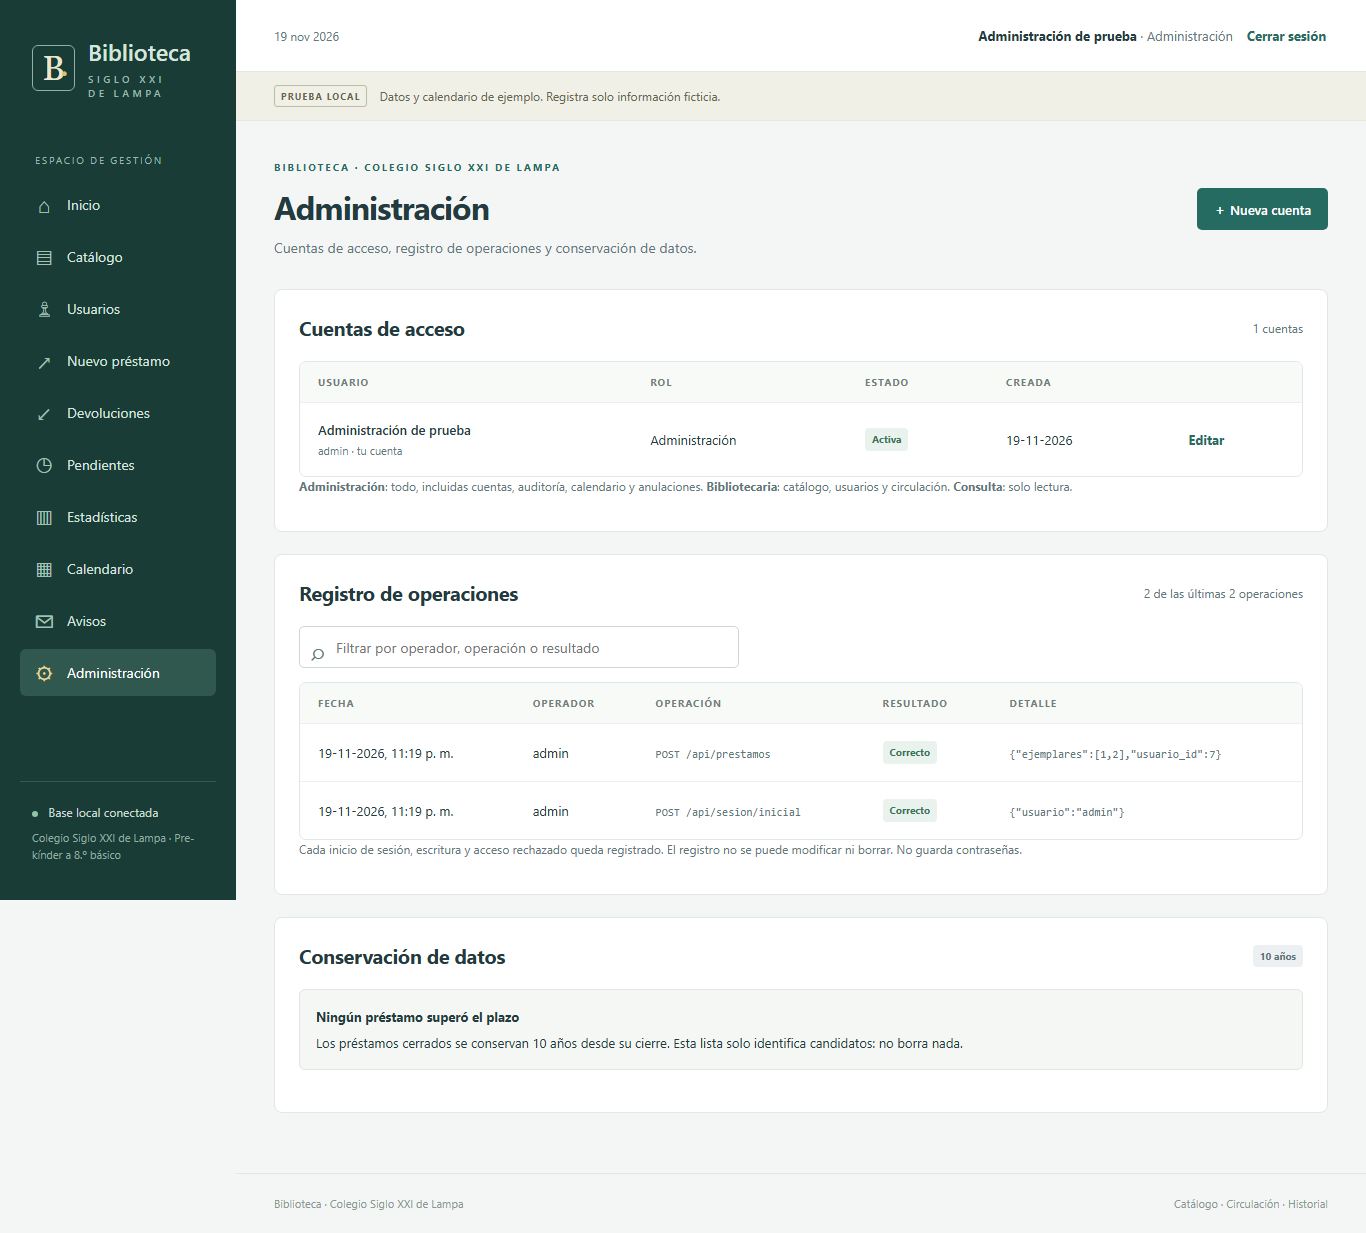
\includegraphics[width=0.85\textwidth]{api-administracion.png}
\caption{Pantalla de administración: el registro de operaciones (\texttt{GET /api/auditoria}) muestra la cuenta inicial y el préstamo válido de P8, ambos con resultado correcto.}
\label{fig:api-admin}
\end{figure}


\subsection{Análisis y hallazgos}
\textbf{Resultado esperado de la solución.} Agilizar el catálogo y mantener el control de los préstamos:
\begin{itemize}[nosep]
\item \textbf{Catálogo:} autocompletar los datos disponibles y revisarlos antes de guardar, reduciendo la digitación.
\item \textbf{Operaciones:} consultar ejemplares disponibles, pendientes y atrasados.
\item \textbf{Historial:} conservar los movimientos y obtener estadísticas anuales.
\end{itemize}

\textbf{Decisiones de diseño que cambiaron.} El modelo presentado en el avance tenía diez entidades y el implementado tiene 20; al implementar las reglas aparecieron necesidades que no cabían en él. Los días hábiles no se pueden calcular sin saber qué días atiende la biblioteca, así que se agregó la tabla \texttt{calendario}. Las pérdidas y los daños necesitaban su propio registro (\texttt{incidencia}) para no inventar devoluciones falsas. El curso se guardó en el préstamo (\texttt{curso\_al\_prestar\_id}), porque con el curso actual el KPI 1 cambiaría cada año. El historial pasó a ser inmutable: un error se corrige con una anulación y no con un \texttt{UPDATE}.

\textbf{Dificultades.} La más relevante fue que varias reglas (máximo de ejemplares simultáneos, préstamo con al menos un detalle, renovación antes del vencimiento) no se pueden expresar con restricciones declarativas, y hubo que implementarlas con triggers, incluso diferidos. También costó separar los atributos derivados de los datos históricos para justificar que no rompen 3FN.

\textbf{KPIs con los datos de ejemplo (2026).} Préstamos por curso: 5.º básico 3, 6.º básico 3 y sin curso 1. Libro más prestado: «Obra ficticia 1», con 2 ejemplares retirados.

\textbf{Cumplimiento de las reglas.} Las 19 reglas quedan implementadas en la base (restricciones, triggers o procedimientos) y cada una tiene al menos una prueba automática; la trazabilidad completa está en \texttt{docs/normalizacion.md} del repositorio.

%------------------------------------------------------------
\section{Conclusión}
Se diseñó e implementó una base de datos relacional para la biblioteca del Colegio Siglo XXI de Lampa, que gestiona catálogo, ejemplares, usuarios y movimientos, y que completa los datos bibliográficos desde Google Books a partir del ISBN. El objetivo general se cumplió: la base responde a los requerimientos levantados y cada decisión de diseño quedó documentada y justificada en este informe.

Respecto de los objetivos específicos:
\begin{enumerate}[nosep]
\item Se documentaron 19 reglas de negocio y los supuestos asumidos (Sección~3.1). Como el caso es hipotético, no hay actas ni correos de un cliente real (Anexos A--C).
\item Se construyó el modelo E-R en notación pata de gallo, con cardinalidad y opcionalidad justificadas en ambos extremos (Sección~3.2).
\item Se transformó al modelo relacional siguiendo los siete pasos del algoritmo y se normalizó: todas las relaciones están en 3FN y la mayoría en FNBC (Secciones~3.3 y 3.4).
\item Se implementó el modelo físico en PostgreSQL, se pobló con datos ficticios y se agregaron triggers, procedimientos almacenados y una API web, todo verificado con pruebas (Secciones~3.5 a 3.7 y 4).
\item El trabajo se comunica en este informe y en la presentación ejecutiva.
\end{enumerate}
Como trabajo futuro quedan la migración de los datos reales desde ABIES, con autorización del colegio, y el envío programado de los avisos de atraso.

%------------------------------------------------------------
\begin{thebibliography}{9}
\bibitem{elmasri} R. Elmasri y S. B. Navathe, \textit{Fundamentals of Database Systems}, 7.ª ed. Pearson, 2016.
\bibitem{silberschatz} A. Silberschatz, H. F. Korth y S. Sudarshan, \textit{Database System Concepts}, 7.ª ed. McGraw-Hill, 2019.
\bibitem{ley21719} Congreso Nacional de Chile, «Ley N.º 21.719, que regula la protección y el tratamiento de los datos personales y crea la Agencia de Protección de Datos Personales», \textit{Diario Oficial de la República de Chile}, 2024.
\bibitem{gbusing} Google, «Using the API (Google Books APIs v1)». \url{https://developers.google.com/books/docs/v1/using}
\bibitem{gbvolumes} Google, «Volumes (Google Books APIs v1 reference)». \url{https://developers.google.com/books/docs/v1/reference/volumes}
\end{thebibliography}

%------------------------------------------------------------
\appendix
\section*{Anexos}

\subsection*{Anexo A. Autorización del cliente}
No aplica. El caso es hipotético: no se usó información del colegio ni de personas reales, y todos los datos de la base son inventados (Sección~\ref{sec:tratamiento}).

\subsection*{Anexo B. Minutas de reuniones}
No hubo reuniones con un cliente real. Las decisiones del grupo quedaron en la presentación de avance y, durante la implementación, en el historial de cambios del repositorio.

\subsection*{Anexo C. Correos y supuestos}
No hubo correos con un cliente. Los supuestos asumidos están en la Sección~3.1 (Supuestos).

\subsection*{Anexo D. Código extenso}
El script completo (936 líneas) se entrega aparte como \texttt{BibliotecaSigloXXI-scripts.sql}, en el mismo archivo comprimido que este informe. Contiene, en orden: esquema y tablas, reglas (triggers), procedimientos, datos de ejemplo, administración del calendario, devolución con condiciones, avisos, anulación de préstamos, seguridad y auditoría, cursos del colegio y consultas de ejemplo. También está en la carpeta \texttt{sql/} del repositorio.

\subsection*{Anexo E. Tablas grandes}
\textbf{Volumen de poblamiento por tabla.}

{\small
\begin{tabular}{@{}l r l r l r@{}}
\toprule
\textbf{Tabla} & \textbf{Filas} & \textbf{Tabla} & \textbf{Filas} & \textbf{Tabla} & \textbf{Filas}\\
\midrule
editorial & 2 & curso & 20 & detalle\_devolucion & 5\\
autor & 3 & usuario & 12 & incidencia & 2\\
genero & 3 & calendario & 730 & sancion & 1\\
libro & 12 & prestamo & 6 & aviso\_correo & 1\\
libro\_autor & 13 & detalle\_prestamo & 9 & correccion & 0\\
libro\_genero & 12 & renovacion & 1 & operador, auditoria & 0\\
ejemplar & 37 & devolucion & 5 & control\_operacion & 1\\
\bottomrule
\end{tabular}}

Las cuentas (\texttt{operador}) y la auditoría empiezan vacías: la primera cuenta se crea al abrir la aplicación. El diccionario de datos completo (tablas, columnas, tipos y claves) corresponde a la Figura~2 y al documento \texttt{BibliotecaSigloXXI-modelos.pdf}.

\end{document}

